\documentclass[11pt,twoside]{report}
\usepackage{lmodern}
\usepackage{amssymb,amsmath}
\usepackage{ifxetex,ifluatex}
\usepackage{fixltx2e} % provides \textsubscript
\ifnum 0\ifxetex 1\fi\ifluatex 1\fi=0 % if pdftex
  \usepackage[T1]{fontenc}
  \usepackage[utf8]{inputenc}
\else % if luatex or xelatex
  \ifxetex
    \usepackage{mathspec}
    \usepackage{xltxtra,xunicode}
  \else
    \usepackage{fontspec}
  \fi
  \defaultfontfeatures{Mapping=tex-text,Scale=MatchLowercase}
  \newcommand{\euro}{€}
\fi
% use upquote if available, for straight quotes in verbatim environments
\IfFileExists{upquote.sty}{\usepackage{upquote}}{}
% use microtype if available
\IfFileExists{microtype.sty}{%
\usepackage{microtype}
\UseMicrotypeSet[protrusion]{basicmath} % disable protrusion for tt fonts
}{}
\usepackage[margin=1in]{geometry}
\usepackage{graphicx}
\makeatletter
\def\maxwidth{\ifdim\Gin@nat@width>\linewidth\linewidth\else\Gin@nat@width\fi}
\def\maxheight{\ifdim\Gin@nat@height>\textheight\textheight\else\Gin@nat@height\fi}
\makeatother
% Scale images if necessary, so that they will not overflow the page
% margins by default, and it is still possible to overwrite the defaults
% using explicit options in \includegraphics[width, height, ...]{}
\setkeys{Gin}{width=\maxwidth,height=\maxheight,keepaspectratio}
\ifxetex
  \usepackage[setpagesize=false, % page size defined by xetex
              unicode=false, % unicode breaks when used with xetex
              xetex]{hyperref}
\else
  \usepackage[unicode=true]{hyperref}
\fi
\hypersetup{breaklinks=true,
            bookmarks=true,
            pdfauthor={},
            pdftitle={},
            colorlinks=true,
            citecolor=blue,
            urlcolor=blue,
            linkcolor=magenta,
            pdfborder={0 0 0}}
\urlstyle{same}  % don't use monospace font for urls
\setlength{\parindent}{0pt}
\setlength{\parskip}{6pt plus 2pt minus 1pt}
\setlength{\emergencystretch}{3em}  % prevent overfull lines
\setcounter{secnumdepth}{0}

%%% Use protect on footnotes to avoid problems with footnotes in titles
\let\rmarkdownfootnote\footnote%
\def\footnote{\protect\rmarkdownfootnote}

%%% Change title format to be more compact
\usepackage{titling}

% Create subtitle command for use in maketitle
\newcommand{\subtitle}[1]{
  \posttitle{
    \begin{center}\large#1\end{center}
    }
}

\setlength{\droptitle}{-2em}
  \title{}
  \pretitle{\vspace{\droptitle}}
  \posttitle{}
  \author{}
  \preauthor{}\postauthor{}
  \date{}
  \predate{}\postdate{}

\usepackage[english,brazilian]{babel} % suporte para línguas
\usepackage[utf8] {inputenc} % codificação

\usepackage{subfig, epsfig}
\captionsetup[subfigure]{style=default, 
  margin=0pt, parskip=0pt, hangindent=0pt, indention=0pt, 
  singlelinecheck=true, labelformat=parens, labelsep=space}

\usepackage{ae}
\usepackage{aecompl}
\usepackage{booktabs}
\usepackage[T1] {fontenc}

\usepackage{footnote}

% Notas criadas nas tabelas ficam no fim das tabelas
\makesavenoteenv{tabular}

\usepackage{fancyhdr}

\fancypagestyle{plain}
{
  \fancyhf{}%
  \renewcommand{\headrulewidth}{0pt}%
  \fancyfoot[C]{\thepage}
}

\usepackage{graphicx,wrapfig} % para incluir figuras
\usepackage[all]{xy} % para incluir diagramas
\usepackage{amsfonts, amssymb, amsthm, amsmath, amscd, textcomp} % pacote AMS
\usepackage{color, float, bbm, multicol, rotating}
\usepackage{verbatim, listings, booktabs}

\usepackage{caption} % Customizar as legendas de figuras e tabelas
\usepackage{array} % Elementos extras para formatação de tabelas

\usepackage{lineno} % números nas linhas

\usepackage {tocvsec2} % controlar profundidade de table of contents
\setcounter {secnumdepth}{0}
\setcounter {tocdepth}{1}

%\widowpenalty10000
%\clubpenalty10000

\usepackage{mathpazo} % fonte palatino
\usepackage{hyperref}

% Adicionar bibliografia, índice e conteúdo na Tabela de conteúdo
% Não inclui lista de tabelas e figuras no índice
\usepackage[nottoc,notlof,notlot, notindex]{tocbibind}

\usepackage{icomma} % Posicionar inteligentemente a vírgula como separador decimal
\usepackage[tight]{units} % Formatar as unidades com as distâncias corretas

\usepackage{setspace}

\usepackage{lastpage} % Conta o número de páginas

\usepackage{pdflscape} % ambiente landscape

\usepackage[round]{natbib}
\usepackage{chapterbib}

\usepackage[flushleft]{threeparttable}
\usepackage {tabularx}

\usepackage[draft]{pdfpages}

\usepackage[draft]{fixme}
%\usepackage{pdfcomment}

\fxsetup{layout={footnote}}

% --- definições gerais ---
\newcommand{\barra}{\backslash}
\newcommand{\To}{\longrightarrow}
\newcommand{\abs}[1]{\left\vert#1\right\vert}
\newcommand{\set}[1]{\left\{#1\right\}}
\newcommand{\seq}[1]{\left<#1\right>}
\newcommand{\norma}[1]{\left\Vert#1\right\Vert}
\newcommand{\hr}{\par\noindent\hrulefill\par}
% --- ---

\newcommand{\titulo}{Perspectivas sobre o reconhecimento de padrões de modularidade e suas implicações para a evolução de morfologias complexas}
\newcommand{\nomedoaluno}{Guilherme Garcia}
\newcommand{\advisor}{Gabriel Marroig} \newcommand{\ano}{2015}
\hypersetup{colorlinks=true, linkcolor=black, citecolor=black,
  filecolor=black, pagecolor=black, urlcolor=black,
  pdfauthor={\nomedoaluno}, pdftitle={\titulo}, pdfsubject={Genética e
    Biologia Evolutiva}, pdfkeywords={Genética Quantitiva, Morfologia
    Craniana, Roedores}, pdfproducer={Latex}, pdfcreator={pdflatex}}
 
\geometry{bindingoffset=15pt}
%\geometry{paperwidth=290mm, paperheight=297mm, margin=1in}
%\setlength{\marginparwidth=80mm}


\begin{document}

\maketitle


% Capa
\begin{titlepage}
\begin{center}
\par
\LARGE {\bf \nomedoaluno} \\
\vspace\fill
\Huge {\titulo} \\
\vspace\fill \Large {On the recognition of modularity patterns and its implications for the evolution of complex morphologies} \\
\vspace\fill
\Large {\bf \advisor} \\
\large {Orientador} \\
\vspace\fill
{\bf{\large São Paulo}\\
  {\large \ano}}
\end{center}
\end{titlepage}

\pagestyle{empty}
\newpage
\cleardoublepage

\pagestyle{plain}

% Números das páginas em algarismos romanos
\pagenumbering{roman}

% Página de Rosto
\begin{center}
\LARGE{\nomedoaluno}
\par
\vspace\fill
\Huge {\titulo}
\end{center}
\par
\vspace\fill \hspace*{150pt}\parbox{10cm}{{\large Tese
    apresentada ao Instituto de Biociências da Universidade de São
    Paulo, para a obtenção de Título de Doutor em Ciências, na Área de
    Genética e Biologia Evolutiva.}}

\par
\vspace {1 cm}
\hspace*{150pt}\parbox{10cm}{{\large Orientador: \advisor}}

\par
\vspace\fill
\begin{center}
\textbf{{\large São Paulo}\\
{\large \ano}}
\end{center}

\newpage

% Ficha Catalográfica
\begin {center}
Ficha Catalográfica \\
\fbox{
  \begin{minipage}{10cm}
    Garcia, Guilherme

    \hspace{2em} \titulo.

    \hspace{2em} \pageref{LastPage} páginas.
    
    \hspace{2em}Tese (Doutorado) - 
    Instituto de Biociências da Universidade de São Paulo. 
    Departamento de Genética e Biologia Evolutiva.
    
    \begin{enumerate}
    \item Evolução Morfológica;
    \item Morfologia Craniana;
    \item Modularidade;
    \item Integração Morfológica;
    \item Primatas Antropóides.
    \end{enumerate}
    I. Universidade de São Paulo. 
    Instituto de Biociências. 
    Departamento de Genética e Biologia Evolutiva.
  \end{minipage}
}
\par
\vspace\fill
{\LARGE\textbf{Comissão Julgadora:}}

\par
\vspace\fill
\begin{tabular*}{\textwidth}{@{\extracolsep{\fill}}l l}
\rule{16em}{1px} 	& \rule{16em}{1px} \\
Prof. Dr. 		& Prof. Dr. \\
 & \\
\end{tabular*}

\par
\vspace\fill
\begin{tabular*}{\textwidth}{@{\extracolsep{\fill}}l l}
\rule{16em}{1px} 	& \rule{16em}{1px} \\
Prof. Dr. 		& Prof. Dr. \\
 & \\
\end{tabular*}

\par
\vspace\fill

\parbox{16em}{\rule{16em}{1px} \\
Prof. Dr. \advisor}
\end{center}

\newpage

% Dedicatória
% Posição do texto na página
\vspace*{0.75\textheight}
\begin{flushright}
  \emph{Para Moisés e Ramiro.}
\end{flushright}

\newpage

% Epígrafe
\vspace*{0.2\textheight}
{\noindent 
If only I could \\
Clear my eyes \\
Then I might breathe once more \\
Then I might breathe again \\
\vspace{0.2 cm} \\
Old sun and stars, \\
And oceans below me \\
Guide my strides over \\
Jagged shards, under foot \\
\vspace{0.2 cm} \\
To slash to the sound \\
How many sit on woe or peril? \\
How many walk on their own? \\
\vspace{0.2 cm} \\
Into the truth \\
Let myself burn \\
Now it's written \\
1000 shards \\
}
\begin{flushright}
\emph {Isis - 1000 Shards}
\end{flushright}

\newpage

% Agradecimentos

% Espaçamento duplo

% \noindent{\LARGE\textbf{Agradecimentos}}

% \vspace{1.0 cm} 
% \emph{``If I have seen further, it is by standing in
%   the shoulder of giants.''}
% \begin{flushright}
% \emph {Isaac Newton}
% \end{flushright}
% \vspace{1.0 cm}
% \noindent{
%   \onehalfspacing

Em primeiro lugar, agradeço ao meu orientador, Gabriel Marroig, por ter me dado a oportunidade de trabalhar neste tema e por sempre contribuir para me devolver ao chão com as nossas discussões e o rigor com que ele encara a ciência. 
Espero que nós tenhamos muitos e muitos anos de colaboração pela frente.

Agradeço também aos meus pares, os demais alunos do LEM, por prover um ambiente fantástico para se fazer ciência, onde as discussões sempre acontecem, inclusive agora, aqui ao lado, enquanto escrevo estes agradecimentos. 
E claro, muitas vezes nossas discussões vão para além da ciência, mas nunca em direção ao senso comum, e estas outras conversas também contribuem ao seu modo para a confecção de um doutor em ciências.

À Aninha, por ser diversas vezes interrompida por um fluxo caótico de ideias inacabadas e ter a paciência de escutá-las, desvantagem de sentar ao meu lado.
À Paulinha, por nunca ter recusado ir tomar um café comigo, mesmo que ela precisasse muito ir embora e por toda a empolgação que ela traz em relação a tudo que a gente faz.
À Dani, pelo suprimento infinito de polenguinho light, por ler vários pedaços desta tese ainda em formação, e por todos os sorrisos e abraços que ajudaram nas horas mais escuras.
À Tafinha (ou Bárbara), por manter o bom humor mesmo nestas horas escuras e por sempre estar disposta a discutir essencialmente qualquer coisa, independente de quanto tempo isso vai levar.
À Monique, pelas divagações aleatórias a respeito de ciência, que contribuem muito pra esta tese, sem dúvida, e também pelas conversas a respeito das nossas crianças lindas.
Ao Ogro (ou Diogo), pela parceria agora de longa data nas partes mais cabeludas das análises e por ser uma fonte inesgotável de boa música, boa comida, e bom gosto em geral.
Ao Lugar (ou Fábio), pelo humor \emph{nonsense} afiadíssimo que sempre alegra o dia e pelas nossas discussões edificantes a respeito do mundo mágico da morfometria geométrica.
Ao Wally (ou Thiago), pela companhia nas tarefas mais divertidas, por exemplo levar computadores pro conserto, e claro, pelas infinitas discussões sobre ciência, sociedade e muito, muito mais.
E à Papete (ou Anna), por ser uma boa companhia pra todas as horas, da mesinha até a volta pra casa, por escutar o que eu tenho a dizer, independente do que seja, e pelas parcerias que a gente ainda deve levar em frente a respeito desses primatas aí.
Também agradeço aqueles que já deixaram o LEM, em especial Alex, Fino, Edgar e Harley, por todas as contribuições pessoais e profissionais nos anos que passaram.
Nesse embalo, agradeço também o Aríete (ou Gustavo) pelas nossas discussões regadas à café ou cerveja, que com certeza contribuem muito, e também por ler pedaços desta tese em formação.

Agradeço também aos colegas do grupo-irmão do Diogo Meyer, que ofereçem diversas perspectivas diferentes às nossas; em especial à Bárbara e ao Limão (ou Luiz Carlos), pelas conversas muito boas que tivemos recentemente. Também agradeço ao Rui Murrieta, pela oportunidade de ser monitor na disciplina de Filosofia, o que certamente contribuiu para o desenvolvimento desta tese, e ao Sérgio Matioli, por conta dos comentários durante a minha qualificação que foram o ponto de partida para o Capítulo 4. 

Agradeço à FAPESP pela concessão de uma bolsa de doutorado.

Devo também agradecer a minha família. 
Sem todos vocês, seria impossível chegar até aqui. 
Em especial, aos meus pais, Eduardo e Teresa, pelo apoio incondicional durante todos esses anos.
Ao meu irmão Gustavo, que nunca tem receios em me dizer o que eu tenho que ouvir.
E à vó Carlota, pela dieta de banana, cabeça de peixe e taboada na infância.

Finalmente, agradeço a minha companheira, a Giuliana, por estar aqui ao meu lado, mesmo nos piores momentos, e por me oferecer aquele abraço perfeito.
E ao Ramiro, nosso menininho, por conta daquele sorriso lindo que ele deu ontem quando eu cheguei em casa, e por dar tanto sentido a tudo.

\singlespacing
% }

\newpage

\vspace*{10pt}
\begin{center}
  \emph{\begin{large}Resumo\end{large}}\label{resumo}
\vspace{2pt}
\end{center}

\noindent
\par
\vspace{1em}
\noindent\textbf{Palavras-chave:} evolução morfológica, morfologia craniana, 
modularidade, integração morfológica, primatas antropóides

\newpage
\vspace*{10pt}
\begin{center}
  \emph{\begin{large}Abstract\end{large}}\label{abstract}
\vspace{2pt}
\end{center}

\selectlanguage{english}
\noindent

\par
\vspace{1em}
\noindent\textbf{Keywords:} morphological evolution, cranial morphology, 
modularity, morphological integration, anthropoid primates

\selectlanguage{brazilian}

\newpage

% Índice
\tableofcontents
%\listoffigures
%\listoftables
\newpage

\pagenumbering{arabic}

\def\sectionautorefname{Seção}
\def\chapterautorefname{Capítulo}
\def\figureautorefname{Figura}
\def\tableautorefname{Tabela}

\onehalfspacing

\pagestyle{fancy}

\renewcommand{\chaptermark}[1]{\markboth{#1}{}}
\renewcommand{\sectionmark}[1]{\markright{#1}{}}

\fancyhf{} \fancyhead[RO]{\leftmark} \fancyhead[LE]{\rightmark}
\fancyfoot[C]{\thepage}

\renewcommand{\headrulewidth}{0.5pt}

\newpage
\chapter{Introdução}
\label{ch:intro}

\begin {sidewaystable} [htp]
  \caption {Vinte e dois marcos anatômicos registrados no crânio de antropóides. As regiões e sub-regiões cranianas às quais cada marco anatômico pertence também estão indicadas. A vista na qual cada marco foi registrado está indicada por A (anterior), P (posterior) ou AP (ambas). As descrições em itálico correspondem a marcos anatômicos tomados sobre a linha sagital. \label {tab:lms}}
  \centering
  \begin {tabularx} {\textwidth} { l c p{3 cm} p{5.5 cm} X }
    \toprule
    {\bf Marco} & {\bf Posição} & {\bf Região} & {\bf Sub-região} & {\bf Descrição} \\
    \midrule
    IS & A & Face & Oral/Nasal
    & {\it interincisivo superior}
    \\
    PM & A & Face & Oral
    & sutura maxilar-premaxilar 
    \\
    NSL & A & Face & Nasal/Oral
    & {\it extremidade rostral do osso nasal} 
    \\
    NA & A & Face & Nasal/Órbita
    & {\it extremidade caudal do osso nasal (junção com o osso frontal)} 
    \\
    BR & AP & Neurocrânio & Abóbada
    & {\it sutura entre o frontal e o parietal (posição medial)} 
    \\
    PT & AP & Neurocrânio & Abóbada 
    & sutura entre o frontal e o parietal 
    \\
    FM & A & Face & Zigomático/Órbita
    & fronto-malar 
    \\
    ZS & A & Face & Oral/Zigomático/Órbita
    & sutura superior entre o zigomático e o maxilar 
    \\
    ZI & A & Face & Zigomático 
    & sutura inferior entre o zigomático e o maxilar 
    \\
    MT & A & Face & Oral
    & tuberosidade maxilar caudal ao terceiro molar 
    \\
    PNS & A & Face & Oral
    & {\it espinha caudal do nasal} 
    \\
    APET & A & Neurocrânio & Base
    & petrous temporal 
    \\
    BA & AP & Neurocrânio & Base
    & {\it ponto ventral do forame magno} 
    \\
    OPI & AP & Neurocrânio & Base/Abóbada
    & {\it ponto dorsal do forame magno} 
    \\
    EAM & A & Neurocrânio & Zigomático/Abóbada
    & meato auditivo externo rostral 
    \\
    PEAM & A & Neurocrânio & Abóbada 
    & meato auditivo esterno caudal 
    \\
    ZYGO & A & Face & Zigomático 
    & sutura entre o zigomático e o temporal 
    \\
    TSP & A & Neurocrânio & Zigómatico/Base/Abóbada
    & sutura entre o temporal o esfenoidal e o frontal 
    \\
    TS & AP & Neurocrânio & Base 
    & sutura entre o temporal e o esfenoidal 
    \\
    JP & AP & Neurocrânio & Base 
    & processo jugular 
    \\
    LD & P & Neurocrânio & Abóbada
    & {\it sutura entre o occipital e o interparietal na linha média} 
    \\
    AS & P & Neurocrânio & Abóbada 
    & sutura entre o parietal e o occipital 
    \\
    \bottomrule
  \end {tabularx}
\end {sidewaystable}

\begin{figure}[htbp]
\centering
\includegraphics{Figures/landmarks.png}
\caption{Configuração de Marcos Anatômicos. As linhas conectando os
marcos indicam os caracteres considerados, tanto sob a forma de
distâncias euclidianas quanto variáveis locais de forma. Linhas
pontilhadas e tracejadas indicam a associação dos caracteres às
hipóteses \emph{a priori} de integração (Face e Neurocrânio,
respectivamente). \label{fig:landmarks}}
\end{figure}

\begin {table}[hp]
  \centering
  \caption {As 38 distâncias euclidianas calculadas sobre os marcos anatômicos e as regiões e sub-regiões às quais cada caráter pertence. \label{tab:dist}}
  
  \hr
  \begin {tabularx} {\textwidth} {X X X}
    \bf{Distância} & \bf{Região} & \bf{Sub-região}  \\
    \hline
    IS.PM & Face & Oral \\
    IS.NSL & Face & Nasal \\
    IS.PNS & Face & Oral/Nasal \\
    PM.ZS & Face & Oral \\
    PM.ZI & Face & Oral \\
    PM.MT & Face & Oral \\
    NSL.NA & Face & Nasal \\
    NSL.ZS & Face & Nasal \\
    NSL.ZI & Face & Oral/Nasal \\
    NA.BR & Neurocrânio & Abóbada \\
    NA.FM & Neurocrânio & Órbita \\
    NA.PNS & Face & Nasal \\
    BR.PT & Neurocrânio & Abóbada \\
    BR.APET & Neurocrânio & Abóbada \\
    PT.FM & Neurocrânio & Órbita \\
    PT.APET & Neurocrânio & Abóbada \\
    PT.BA & Neurocrânio & Abóbada \\
    PT.EAM & Neurocrânio & Abóbada \\
    PT.ZYGO & Face & Zigomático \\
    FM.ZS & Neurocrânio & Órbita \\
    ZS.ZI & Face & Oral \\
    ZI.MT & Face & Oral \\
    ZI.ZYGO & Face & Zigomático \\
    ZI.TSP & Face & Zigomático \\
    MT.PNS & Face & Oral \\
    PNS.APET & Neurocrânio & Base \\
    APET.BA & Neurocrânio & Base \\
    APET.TS & Neurocrânio & Base \\
    BA.EAM & Neurocrânio & Base \\
    EAM.ZYGO & Face & Zigomático \\
    ZYGO.TSP & Face & Zigomático \\
    LD.AS & Neurocrânio & Abóbada \\
    BR.LD & Neurocrânio & Abóbada \\
    OPI.LD & Neurocrânio & Abóbada \\
    PT.AS & Neurocrânio & Abóbada \\
    JP.AS & Neurocrânio & Base \\
    BA.OPI & Neurocrânio & Base \\
  \end {tabularx}
  \hr
\end {table} % sk:tab:dist

\begin{figure}[htbp]
\centering
\includegraphics{Figures/phylo_model-1.pdf}
\caption{Tamanhos amostrais e efeitos fixos controlados para as 109 OTUs
de primatas antropóides. \label{fig:phylo_model}}
\end{figure}

\def\sectionautorefname{Section} \def\chapterautorefname{Chapter}
\def\figureautorefname{Figure} \def\tableautorefname{Table}

\selectlanguage{english}

\newpage
\chapter{Type I and II Error Rates in Modularity Hypothesis Testing}
\label{ch:modcomp}

\textsuperscript{1}Laboratório de Evolução de Mamíferos, Departamento de
Genética e Biologia Evolutiva, Instituto de Biociências, Universidade de
São Paulo, CP 11.461, CEP 05422-970, São Paulo, Brasil

\textsuperscript{2}\href{mailto:wgar@usp.br}{wgar@usp.br}

running title: Error in Modularity Hypothesis Testing

key words:

\section{Introduction}\label{introduction}

Modularity is a characteristic pattern that biological systems exhibit
concerning the distribution of interactions between their composing
elements; that is, in a given system, certain subsets of elements,
denominated modules, interact more among themselves than with other such
subsets (Newman, 2006; Mitteroecker \& Bookstein, 2007; Wagner \emph{et
al.}, 2007; Klingenberg, 2008). This pattern has been well documented at
different levels of biological organization, from the dynamics of
metabolic networks ({\textbf{???}}; e.g. Ravasz \emph{et al.}, 2002) to
the structure of interactions among individuals in populations (e.g.
{\textbf{???}}) and among species in ecological communities (e.g.
{\textbf{???}}).

Regarding morphological systems, the concept of modular organization is
nested within the framework of morphological integration (Olson \&
Miller, 1958; Cheverud, 1996a), which refers to the organization of
correlations among morphological elements and the set of hypothesis
concerning their relationships. In this context, modularity refers to a
particular organization of genetic effects over phenotypic variation,
articulated through development (genotype/phenotype map;
{\textbf{???}}). A modular organization of the genotype/phenotype map is
thought to emerge as the result of selection for conflicting functional
demands ({\textbf{???}}); for instance, the decoupling between fore- and
hindlimb function in certain mammalian lineages such as bats
({\textbf{???}}) and apes ({\textbf{???}}) is accompanied with the
modularization of both structures, as shown by a reduction of phenotypic
correlations among limbs and an increase in correlations within limbs.

The recognition of such variational modules ({\textbf{???}}; Wagner
\emph{et al.}, 2007) over covariance or correlation patterns in adult
populations involves a comprehension of the underlying developmental
dynamics. In the mammalian skull, development is composed of sequential
steps that may be regarded as modular in the sense that they are
confined to specific skull regions, such as brain growth or muscle-bone
interactions ({\textbf{???}}; Hallgrímsson \& Lieberman, 2008). However,
these confined steps tend to also affect adjoining regions through
interaction among developing tissues ({\textbf{???}}; Lieberman, 2011;
Esteve-Altava \& Rasskin-Gutman, 2014), and the composed effect of these
different processes over correlation patterns in adult phenotypes may be
misleading ({\textbf{???}}; Hallgrímsson \emph{et al.}, 2009).
Furthermore, of particular importance in the context of mammalian
morphological systems is variation in overall growth rates, which, in
adult populations, emerges into size variation (Porto \emph{et al.},
2013). This source of variation affects the overall level of phenotypic
correlations among morphological traits ({\textbf{???}}; Wagner, 1984),
and the magnitude of overall integration has important consequences for
both the evolution of mean phenotypes among species (e.g.
{\textbf{???}}, {\textbf{???}}) and the evolution of morphological
integration itself (Oliveira \emph{et al.}, 2009; Porto \emph{et al.},
2009, 2013; Shirai \& Marroig, 2010).

In the present work, we compare the methods described both by Cheverud
et al. (1989) and Klingenberg (2009) to test \emph{a priori} defined
modularity patterns, using anthropoid primates as a model organism. In
order to also compare the performance of these methods with respect to
different representations of form, sample units are represented both as
interlandmark distances and shape variables. Furthermore, we also used
an approach based on the construction of theoretical correlation
matrices; in this context, these matrices are used in order to estimate
Type I and Type II error rates for both methods. Since these methods
were designed under different frameworks, the present work also puts
some effort into unifying both methods into the same conceptual and
statistical framework, in order to produce meaningful comparisons.

\section{Methods}\label{methods}

\subsection{Sample}\label{sample}

The database used here (\autoref{tab:modcomp_otu}) consists of 21
species, distributed across all taxonomic denominations of Anthropoidea
above the genus level. These OTUs were selected from a broader database
(Marroig \& Cheverud, 2001; Oliveira \emph{et al.}, 2009) in order to
reduce the effects of low sample sizes over estimates of modularity
patterns. Individuals in our sample are represented by 36 registered
landmarks, using either a Polhemus 3Draw or a Microscribe 3DS for
Platyrrhini and Catarrhini, respectively. Twenty-two unique landmarks
represent each individual (\autoref{fig:landmarks}, \autoref{tab:lms}),
since 14 of the 36 registered landmarks are bilaterally symmetrical. For
more details on landmark registration, see Marroig \& Cheverud (2001)
and Oliveira et al. (2009).

\begin{table}[t]
  \centering
  \begin{threeparttable}
    \caption{Twenty-one species used in the present work, along with sample sizes and linear models adjusted. \label{tab:modcomp_otu}}
    \begin{tabular}{lccr}
        \toprule
        Species & Group$^a$ & $n$ & Model$^b$ \\ 
      \midrule
        \emph{Alouatta belzebul} & P & 109 & X \\ 
        \emph{Ateles geoffroyi} & P & 78 & - \\ 
        \emph{Cacajao calvus} & P & 48 & S + X \\ 
        \emph{Callicebus moloch} & P & 93 & X \\ 
        \emph{Callithrix kuhlii} & P & 129 & - \\ 
        \emph{Cebus apella} & P & 110 & X \\ 
        \emph{Cercopithecus ascanius} & C & 61 & X \\ 
        \emph{Chiropotes chiropotes} & P & 56 & X \\ 
        \emph{Chlorocebus pygerythrus} & C & 110 & X \\ 
        \emph{Colobus guereza} & C & 140 & X \\ 
        \emph{Gorilla gorilla} & C & 115 & X \\ 
        \emph{Homo sapiens} & C & 160 & S * X \\ 
        \emph{Hylobates lar} & C & 66 & X \\ 
        \emph{Macaca fascicularis} & C & 69 & X \\ 
        \emph{Pan troglodytes} & C & 61 & X \\ 
        \emph{Papio anubis} & C & 46 & X \\ 
        \emph{Piliocolobus foai} & C & 83 & X \\ 
        \emph{Pithecia pithecia} & P & 69 & S + X \\ 
        \emph{Procolobus verus} & C & 88 & X \\ 
        \emph{Saguinus midas} & P & 50 & S \\ 
        \emph{Saimiri sciureus} & P & 87 & X \\ 
      \bottomrule
    \end{tabular}
      \begin{tablenotes}
        \footnotesize
        {
        \item[$a$] C: Catarrhini; P: Platyrrhini
        \item[$b$] S: subspecies/population; X: sex.
        }
      \end{tablenotes}
    \end{threeparttable}
  \end{table}


For each OTU, we estimated phenotypic covariance and correlation
matrices for three different types of variables: tangent space
residuals, estimated from a Procrustes superimposition for the entire
sample, using the set of landmarks described on both \autoref{tab:lms}
and \autoref{fig:landmarks} (henceforth refered to as Procrustes
residuals); interlandmark distances, as described in \autoref{tab:dist};
and local shape variables (Márquez \emph{et al.}, 2012), which are
measurements of infinitesimal log volume transformations between each
sample unit and a reference (mean) shape. These transformations were
calculated at 38 points, corresponding to the locations of the mipoints
between pairs of landmarks used to calculate interlandmark distances, in
order to produce a dataset that represents shape (i.e., form without
isometric variation; Bookstein, 1991; Zelditch \emph{et al.}, 2004)
while retaining the same overall properties of the interlandmark
distance dataset, such as dimensionality, for instance. Furthermore, the
same hypotheses of trait association can be used on both types of
variables since the position of local shape variables through the skull
mirrors the position of interlandmark distances, although they are
conceptually different types of measurements.

Here we consider only covariance or correlation structure for the
symmetrical component of variation; therefore, prior to any analysis, we
need to control for variation in assymmetry. For interlandmark
distances, we averaged bilateral measurements within each individual.
For both Procrustes residuals and local shape variables, we follow the
procedure outlined in Klingenberg et al. (2002) for bilateral structures
by obtaning for each individual a symmetrical landmark configuration,
averaging each actual shape with its reflection along the sagittal
plane; we estimate local shape variables afterwards. With respect to
Procrustes residuals, landmarks placed along the sagittal plane will
have zero variation in the direction normal to this plane; we aligned
all specimens' sagittal plane to the $xz$ plane, thus removing the $y$
component for each of these landmarks from covariance/correlation
matrices.

For each dataset, we estimated covariance and correlation matrices after
removing fixed effects of little interest in the present context, such
as sexual dimorphism, for example. For interlandmark distances and local
shape variables, these effects were removed through a multivariate
linear model adjusted for each species, according to
\autoref{tab:modcomp_otu}; for Procrustes residuals, the same effects
were removed by centering all group means to each species' mean shape,
since the loss of degrees of freedom imposed by the GPA prohibits the
use of a full multivariate linear model over this kind of data to
removed fixed effects.

In order to consider the effects of size variation over modularity
patterns, we used a different procedure to remove the influence of size,
according to the different properties of each type of variable. For
interlandmark distances, we use the approach established by Bookstein et
al. (1985); if $\mathbf{C}$ is a correlation matrix, we obtain a
correlation matrix $\mathbf{R}$ without the effect of size using the
equation \[
\mathbf{R} = \mathbf{C} - \lambda_1 v_1 v^{t}_1
\] where $\lambda_1$ and $v_1$ refer respectively to the first
eigenvalue and eigenvector of the spectral decomposition of $C$,
considering that this eigenvector is associated with size variation, a
common pattern in mammalian correlation structure, especially when
interlandmark distances are considered (Wagner, 1984; Mitteroecker
\emph{et al.}, 2004; Mitteroecker \& Bookstein, 2007); $t$ denotes
matrix transpose. For Procrustes residuals and local shape variables,
the effects of isometric variation are removed prior through normalizing
each individual to unit centroid size. However, allometric effects still
influence covariance or correlation structure. In order to remove such
effects, we use a similar procedure, based upon Mitteroecker et al.
(2004), which involves the estimation of an allometric component for
each OTU; this allometric component is related to regression coefficents
for each of the $m$ shape variables (either Procrustes residuals or
local shape variables) over log Centroid Size. If $\mathbf{S}$ is a
covariance matrix, we obtain a covariance matrix $\mathbf{R}$ without
the influence of allometric relationships using the equation \[
\mathbf{R} = (I_m - aa^t) \mathbf{S} (I_m - aa^t)
\] where $a$ refers to the normalized allometric component estimated for
each OTU and $I_m$ represents the identity matrix of size $m$.
Therefore, our empirical dataset consists of six different sets of
covariance/correlation matrices, considering both the nature of
morphometric variables and the presence or absence of variation
associated with size.

\subsection{Empirical Modularity Hypothesis
Tests}\label{empirical-modularity-hypothesis-tests}

Using these six sets of covariance/correlation matrices, we test the
hypotheses of trait associations described in both \autoref{tab:lms} for
Procrustes residuals and \autoref{tab:dist} for interlandmark distances
and local shape variables. These trait sets are grouped with respect to
their scope; two regional sets (Face and Neurocranium), each divided
into three more localized trait sets (Oral, Nasal and Zygomatic for the
Face; Orbit, Base and Vault for the Neurocranium).

For all hypotheses, we estimate both AVG Indexes (Porto \emph{et al.},
2013) and the RV coefficients (Klingenberg, 2009). Both statistics are
estimated by partitioning any given covariance or correlation matrix
into blocks; if $\mathbf{A}$ is a covariance or correlation matrix, the
partition \[
\mathbf{A} =
\begin{bmatrix}
\mathbf{A}_h & \mathbf{A}_b \\
\mathbf{A}^t_b & \mathbf{A}_c
\end{bmatrix}
\] indicates that the block $\mathbf{A}_h$ contains covariances or
correlations between traits that belong to the trait set being
considered, while $\mathbf{A}_c$ represents the complementary set;
$\mathbf{A}_b$ represents the block of covariances or correlations
between the two sets. Thus, covariance ($\mathbf{S}$) or correlation
($\mathbf{C}$) matrices can be partitioned into a similar scheme. We
estimate AVG Indexes using the equation \[
AVGi = \frac {\bar{\rho}_{+} - \bar{\rho}_{-}} {ICV}
\] where $\bar{\rho}_{+}$ represents the average correlation in
$\mathbf{C}_h$, $\bar{\rho}_{-}$ represents the average correlation of
the complementary set (correlations in both $\mathbf{C}_b$ and
$\mathbf{C}_c$), and $ICV$ is the coefficient of variation of
eigenvalues of the covariance matrix, which is a measurement of the
overall integration between all traits (Shirai \& Marroig, 2010). We
estimate RV coefficients for each hypothesis using the relationship \[
RV = \frac{tr(\mathbf{S}_{b}\mathbf{S}^t_{b})}{\sqrt{tr(\mathbf{S}_h \mathbf{S}_h)tr(\mathbf{S}_c \mathbf{S}_c)}}
\] where $tr$ represents the sum of diagonal elements in any given
matrix ($tr \mathbf{A} = \sum_i a_{ii}$).

The partitioning scheme outlined above assumes that the complementary
set does not represent an actual hypothesis of trait association;
however, we may choose to consider that both sets ($\mathbf{A}_h$ and
$\mathbf{A}_c$) represent two distinct hypothesis. The estimation of RV
coefficients remains the same; however, AVG Indexes are estimated
considering that $\bar{\rho}_{+}$ is the average correlation in both
$\mathbf{C}_h$ and $\mathbf{C}_c$, while $\bar{\rho}_{-}$ represents the
average correlation only in $\mathbf{C}_b$. In the particular case of
the distinction between Facial and Neurocranial traits, we also
estimated AVG Indexes in this manner, reporting values for this estimate
under the denomination `Neuroface', following Marroig \& Cheverud
(2001), along independent AVGi estimates for each region. Furthermore,
since both Face and Neurocranium are two disjoint trait sets when any
morphometric variable type is considered, RV coefficient values for
either set are equal; therefore, a single RV value is reported for both
regions, for each variable type.

In order to test the hypothesis that each trait set represent
variational modules, we used a randomization procedure that generates
1000 random trait sets with the same size as the original set,
calculating both AVGi and RV values for each generated set. These values
are used to construct distributions for both statistics that represent
the null hypothesis that a hypothetical trait set is a random
arrangement without meaningful relationships. The value obtained for the
real trait set is then compared to this distribution. In the case of
AVGi, we consider that this null hypothesis is rejected when the real
value is higher than the average value for the null distribution,
considering the significance level established; in the case of RV
coefficient, the null hypothesis is rejected when the real RV value is
lower than the average value for the distribution, also considering a
certain significance level. For Procrustes residuals, the randomization
procedure considers that coordinates within the same landmark should
remain together in each randomly generated trait set, following
Klingenberg \& Leamy (2001).

It is noteworthy that, while the procedure for estimating significance
in the case of AVG Indexes is derived from Mantel's (1967) approach (as
outlined by Cheverud \emph{et al.}, 1989), we chose to generate null
distributions for AVGi directly, instead of estimating matrix
correlation values for both real and permutated matrices. Estimated
$p$-values in both cases remain the same, and the additional step of
estimating matrix correlations would produce an unnecessary difference
between the estimation of signficance for AVGi and RV.

\subsection{Estimation of Error Rates}\label{estimation-of-error-rates}

In order to evaluate the statistical properties of both statistics and
the randomization procedure, we built theoretical correlation matrices
\[
\mathbf{C}_{s} =
\begin{bmatrix}
\mathbf{W}_1 & \mathbf{B} \\
\mathbf{B}^t & \mathbf{W}_2 \\
\end{bmatrix}
\] where $\mathbf{W}_1$ and $\mathbf{W}_2$ represent correlation blocks
associated with two distinct trait sets, and $\mathbf{B}$ represents the
correlation block between both sets.

For each set of empirical correlation matrices used in the previous
section, we obtained average correlation distributions within and
between the trait sets considered (\autoref{fig:cor_dist}). We
constructed corresponding sets of $\mathbf{C}_{s}$ matrices by sampling
each distribution; for each matrix, we sampled two within-set
correlations and one between-set correlation, filling the corresponding
block in the theoretical matrix with the sampled correlations. As an
example with only four traits, divided into two blocks of two traits, if
we sample the values $0.5$ and $0.3$ from the within-set distribution,
and $-0.1$ from the between-set distribution, the corresponding
$\mathbf{C}_{s}$ matrix will be \[
\mathbf{C}_s =
\begin{bmatrix}
1 & 0.5 & -0.1 & -0.1 \\
0.5 & 1 & -0.1 & -0.1 \\
-0.1 & -0.1 & 1 & 0.3 \\
-0.1 & -0.1 & 0.3 & 1 \\
\end{bmatrix}
\] filling each cell in each block with the sampled correlation
associated with that particular block. Thus, we abstract each type of
morphometric variable to a correlation distribution, building
theoretical correlation matrices that are representative of each type
retaining their statistical properties.

\begin{figure}[htbp]
\centering
\includegraphics{Figures/cor_dist-1.pdf}
\caption{Distribution of within-set and between-set correlations derived
from the six types of empirical correlation matrices.
\label{fig:cor_dist}}
\end{figure}

For each of the six pairs of correlation distributions, we built 1000
theoretical correlation matrices for 40 traits; previous tests indicate
that matrix dimensionality does not affect any of our results. We
considered only positive-definite matrices; if any given matrix did not
fit this criterion, we discarded that matrix and sampled a new set of
correlations. This allows us to sample observations from a multivariate
normal distribution using each of these 6000 matrices as the $\Sigma$
parameter. For each matrix, we also sample the size of both trait sets;
we established a minimal value of five traits for the size of any set.

We use this set of 6000 correlation matrices of known structure
($\mathbf{C}_s$) to built another set of correlation matrices of
unknown, random structure ($\mathbf{C}_r$) by simply shuffling both
lines and columns of each matrix; therefore, each $\mathbf{C}_r$ matrix
is associated with a $\mathbf{C}_s$ matrix. For all matrices, both
$\mathbf{C}_r$ and $\mathbf{C}_s$, we obtained samples of increasing
size (20, 40, 60, 80, 100 individuals) and re-estimated a correlation
matrix for each sample, thus also considering in our tests the
uncertainty derived from sampling. For each matrix estimated, both
$\mathbf{C}_r$ and $\mathbf{C}_s$, we test the hypothesis that the two
sets used to generate each $\mathbf{C}_s$ matrix represent two
variational modules, using both AVGi and RV coefficients, as described
in the previous section.

The case in which samples were generated from a $\mathbf{C}_r$ matrix
represents a situation of a true null hypothesis for either tests, since
the correlation matrix used to produce the sample was generated by a
permutation of the hypothesis being tested. Therefore, testing
hypotheses over $\mathbf{C}_r$ matrices allows us to estimate Type I
error rates for both tests, that is, the proportion of cases in which
the null hypothesis is rejected even though it is false, given a
significance level. In an adequate test, we expect that both quantities,
significance level and Type I error rate, will be identical.

The opposite case, when we sampled $\mathbf{C}_s$ matrices, represents a
situation in which we know that the null hypothesis of either tests is
false, since we are testing the hypothesis that the partitioning scheme
used to generate that particular matrix actually represents two
variational modules. Thus, we estimated, in this case, the Type II error
rates, that is, the probability that the null hypothesis is not rejected
even though it is false, given a significance level; here, we represent
Type II error using the power for each test, by simply calculating the
complementar probability to Type II error rate. In an adequate test, we
expect that power will rapidly reach a plateau when significance level
is still close to zero, and further increasing $P(\alpha)$ will not
produce a great increase in power.

Our estimations of power for both statistics should also be controlled
for effect size, since sampled correlations may generate a correlation
structure that is not detected simply due to small differences between
within-set and between-set correlations. For each correlation matrix
sampled, we keep the squared between-set correlation ($b^2$), in order
to use it as an estimate of effect size that is not directly associated
with either AVGi and RV statistics. We expect that power for either
tests will decrease with increasing $b^2$ values, as effect size would
also decrease.

\subsubsection{Software}\label{software}

All analysis were performed under R 3.2.0 (R Core Team, 2015). Source
code for all analyses can be found at \url{http://github.com/wgar84}. It
is noteworthy that previous tests we made indicated no differences
between our estimation of empirical RV coefficients, based upon our own
code, and estimates provided by MorphoJ (Klingenberg, 2011). In order to
obtain symmetrical landmarks configurations, we used code provided by
Annat Haber, available at
\url{http://life.bio.sunysb.edu/morph/soft-R.html}.

\section{Results}\label{results}

\subsection{Empirical Tests}\label{empirical-tests}

Regarding localized trait sets, tests performed using AVG Indexes
(\autoref{fig:MI_Func}) detect a consistent pattern among OTUs for both
interlandmark distances and local shape variables; in the first set, the
Oral sub-region is detected as a modular partition, and, when size is
removed, the Vault sub-region is also detected; both Orbit and Base
region are not detected in any of the tests with this type of variable.
With local shape variables, both Oral and Vault sets are also detected
consistently across OTUs, along Nasal and Zygomatic traits; moreover,
the removal of allometric variation affect only the detection of the
Vault. Notably, the Base sub-region is detected only in 3 of 42 tests.
For Procrustes residuals, the pattern of detection among sub-regions and
OTUs is diffuse; it is noteworthy that the Base sub-region is detected
among several OTUs, which contrasts this type of morphometric variable
with the remaining two types. Furthermore, abstracting the actual tests
performed, \autoref{fig:MI_Func} also indicates that Procrustes
residuals display a low variance for AVGi values within each OTU, while
both interlandmark distances and local shape variables display a
consistent pattern of variation among AVGi values within each OTU, with
lower values for the Base and, for interlandmark distances, Orbit trait
sets.

\begin{figure}[htbp]
\centering
\includegraphics{Figures/MI_Func-1.pdf}
\caption{AVG Index values for localized trait sets. Circles indicate
whether a trait set is recognized as a variational module in a given
OTU, with $P(\alpha)$ indicated by the legend. \label{fig:MI_Func}}
\end{figure}

Tests performed using RV coefficients (\autoref{fig:RV_Func}) show a
more diffuse pattern among each varible type. When interlandmark
distances are considered, most tests detect the Vault sub-region with
size variation retained, and the Base sub-region when size variation is
removed. For Procrustes residuals, few tests are able to reject their
null hypothesis, detecting only a handful of valid modular partitions.
Tests performed on local shape variables display the opposite behavior:
almost all partitions are detected, regardless of whether allometric
variation has been retained or removed. Moreover, RV values display a
pattern of marked variation among OTUs, more so than between values
within each OTU; notably, \emph{Macaca fascicularis} and \emph{Papio
anubis} show RV values much higher than those estimated on remaining
species. This pattern can be observed both on interlandmark distances
with size retained and in Procrustes residuals, although this effect is
more marked in the former type.

\begin{figure}[htbp]
\centering
\includegraphics{Figures/RV_Func-1.pdf}
\caption{RV Coefficient values for localized trait sets. Circles
indicate whether a trait set is recognized as a variational module in a
given OTU, with $P(\alpha)$ indicated by the legend.
\label{fig:RV_Func}}
\end{figure}

With respect to regional trait sets, tests performed using AVGi
(\autoref{fig:MI_Dev}) indicate a pattern consistent with the findings
regarding localized sets (\autoref{fig:MI_Func}). Considering only
interlandmark distances, Facial traits are detected as a valid modular
partition both with size variation retained or removed, while
Neurocranial traits are detected as a valid partition only when size
variation is removed. This pattern mirrors the contrast between Oral and
Vault traits in the localized sets regarding interlandmark distances.
Considering Procrustes residuals, Neurocranial traits are a valid
partition with both size retained and removed; once again, this pattern
mirrors the detection of the Basicranial partition as valid in the
localized sets. Finally, in local shape variables, both Face and
Neurocranium are detected as valid with size retained; with size
removed, only the Face is recognized. The same can be observed in the
localized sets, where removing allometric variation affects the
detection of the Vault set. The tests for distinction between within-set
and between-set correlations for these two sets (designated `Neuroface')
show a pattern that is consistent with tests for the individual sets,
that is, if one of the sets was previously detected, this distinction is
also detected as valid with high probability.

\begin{figure}[htbp]
\centering
\includegraphics{Figures/MI_Dev-1.pdf}
\caption{AVG Index values for regional trait sets. Circles indicate
whether a trait set is recognized in a given OTU, with $P(\alpha)$
indicated by the legend. \label{fig:MI_Dev}}
\end{figure}

Tests performed for this distinction between Face and Neurocranium using
RV coefficients (\autoref{fig:RV_Dev}) show that in most cases, for both
interlandmark distances and local shape variables, both regions are
considered distinct and valid variational modules; in Procrustes
residuals, only in a handful of taxa the same result can be observed. In
this case, the correspondence with results for localized trait sets
(\autoref{fig:RV_Func}) is more difficult, due to the lack of
independent tests for each region.

\begin{figure}[htbp]
\centering
\includegraphics{Figures/RV_Dev-1.pdf}
\caption{RV Coefficient values for regional trait sets. Circles indicate
whether a trait set is recognized in a given OTU, with $P(\alpha)$
indicated by the legend. \label{fig:RV_Dev}}
\end{figure}

\subsection{Error Rates}\label{error-rates}

Comparing the distributions of AVGi and RV values from theoretical
matrices with respect to their structure (\autoref{fig:stat_dist_sim})
shows marked differences between statistics and morphometric variables
from which correlations are sampled. For local shape variables, the
distribution of both AVGi and RV values for $\mathbf{C}_s$ and
$\mathbf{C}_r$ matrices overlap very little; for interlandmark
distances, the distribution of AVGi values for both matrix types also
has little overlap, while the same distributions for RV have a
substantial overlap. Finally, for Procrustes residuals, while the
distribution of AVGi values for both matrix types are overlapping to
some degree, the same distributions for RV values are identical. It is
noteworthy that removing size or allometry does not change these
distributions in most cases; only for RV values estimated over matrices
derived from correlation distributions for interlandmark distances, in
which the removal of size variation increases the overlap in
$\mathbf{C}_s$ and $\mathbf{C}_r$ distributions.

\begin{figure}[htbp]
\centering
\includegraphics{Figures/stat_dist_sim-1.pdf}
\caption{Distribution of AVG Index and RV Coefficient for theoretical
correlation matrices. \label{fig:stat_dist_sim}}
\end{figure}

Regarding the relationship between significance levels and Type I error
rates, estimated over $\mathbf{C}_r$ matrices, \autoref{fig:type1} shows
that these quantities approach an identity relationship very closely,
regardless of whether we use AVGi or RV to quantify variational
modularity; even at low sample sizes, Type I error rates are very close
to significance levels. Furthermore, the effect of sampling correlations
from size-free distributions does not alter Type I error rates for both
tests.

\begin{figure}[htbp]
\centering
\includegraphics{Figures/type1-1.pdf}
\caption{Type I error rates as a function of the chosen significance
level regarding tests for variational modularity applied on
$\mathbf{C}_r$ correlation matrices. The solid black line represents the
identity relationship. \label{fig:type1}}
\end{figure}

When we consider the relationship between power and significance levels,
estimated over $\mathbf{C}_s$ matrices, there are substantial
differences with respect both to the chosen statistic (AVGi or RV) and
to the type of variable from which correlations are sampled. Considering
local shape variables (\autoref{fig:type2_def}), tests using either AVGi
and RV have high power, even at low sample or effect sizes; increasing
these quantities produces a further increase in power. However, it is
noteworthy that, for lower effect sizes (represented by high average
squared correlation between sets, $b^2$) power for tests performed using
AVGi is higher than for those using RV. As effect size increases (lower
$b^2$ values), the difference in power between the two statistics
decreases. For this type of variable, sampling from its associated
size-free correlation distribution implies minor differences in power
for both statistics.

\begin{figure}[htbp]
\centering
\includegraphics{Figures/type2_def-1.pdf}
\caption{Power for both AVGi and RV statistics as a function of the
chosen significance levels with respect to tests for variational
modularity applied on $\mathbf{C}_s$ matrices with values sampled from
the distribution of correlations between local shape variables. Lines
are colored with respect to quantiles of the $b^2$ distribution,
according to the legend. \label{fig:type2_def}}
\end{figure}

For interlandmark distances (\autoref{fig:type2_ed}), there are
substantial differences on the relationship between power and
significance level if we consider the different parameters. First and
foremost, the effect of sampling from the size-free correlation
distribution in order to build $\mathbf{C}_s$ matrices produces a
substantial decrease in power for either tests; however, this decrease
is more pronounced for tests based on the RV statistic, since for lower
effect sizes (high $b^2$ values), power approaches an identity
relationship with significance level. Sample size also interferes with
this relationship, as increasing this quantity also increases power when
higher effect sizes (low $b^2$ values) are considered.

\begin{figure}[htbp]
\centering
\includegraphics{Figures/type2_ed-1.pdf}
\caption{Power for both AVGi and RV statistics as a function of the
chosen significance levels with respect to tests for variational
modularity applied on $\mathbf{C}_s$ correlation matrices with values
sampled from the distribution of correlations between interlandmark
distances. Lines are colored with respect to quantiles of the $b^2$
distribution, according to the legend. The solid black line represents
the identity relationship. \label{fig:type2_ed}}
\end{figure}

With respect to Procrustes residuals (\autoref{fig:type2_sym}), tests
using either AVGi or RV have reduced power, regardless of effect or
sample size. Sampling from size-free correlation distributions to build
$\mathbf{C}_s$ matrices also has little effect. As for interlandmark
distances without size variation, power for tests performed using RV
values approach an identity relationship with significance level;
however, increasing sample size has little effect in this case.

\begin{figure}[htbp]
\centering
\includegraphics{Figures/type2_sym-1.pdf}
\caption{Power for both AVGi and RV statistics as a function of the
chosen significance levels with respect to tests for variational
modularity applied on $\mathbf{C}_s$ matrices with values sampled from
the distribution of correlations between Procrustes residuals. Lines are
colored with respect to quantiles of the $b^2$ distribution, according
to the legend. The solid black line represents the identity
relationship. \label{fig:type2_sym}}
\end{figure}

\section{Discussion}\label{discussion}

\section{References}\label{references}

\newpage
\chapter{Allometric Constraints and Modularity}
\label{ch:allo}

\section{Introduction}\label{introduction-1}

A fundamental feature of morphological systems is their tendency to
exhibit correlations due to commom developmental processes and
functional interactions, a phenomenon called morphological integration
(Olson \& Miller, 1958; Cheverud, 1996a; Hallgrímsson \emph{et al.},
2009). Integration can be characterized both by the magnitude of
correlation between morphological traits and the pattern described by
the inter-trait correlation structure (Marroig \& Cheverud, 2004; Porto
\emph{et al.}, 2013). In mammal morphological systems, traditional
morphometrics analysis of integration emphasize the role of size
variation in determining magnitude of morphological integration and,
through allometric relationships, it is argued that size can also affect
integration patterns (Porto \emph{et al.}, 2009, 2013).

Esta variação de tamanho emerge a partir do processo de crescimento;
ademais, o crescimento heterogêneo de partes distintas em uma dada
estrutura morfológica produz alometria, isto é, a associação entre
qualquer caráter organísmico de interesse e tamanho corporal (Huxley,
1932; Pélabon \emph{et al.}, 2014). É possível definir diferentes tipos
de alometria de acordo com o nível de organização biológica considerado
(Pélabon \emph{et al.}, 2013). Assim, alometria ontogénetica refere-se à
associação entre caracteres e tamanho corpóreo ao longo do
desenvolvimento de um indivíduo; alometria estática refere-se à esta
associação medida em uma população, entre indivíduos em uma mesma faixa
etária; e alometria evolutiva, medida entre médias em populações ou
espécies diferentes. Associações alométricas são classicamente medidas
na escala log (Huxley, 1932; Jolicoeur, 1963); portanto, estabelece-se
uma relação alométrica log-linear entre o caráter $x$ e o tamanho
corporal $m$ da forma \[
\log x = a + b \log m
\] onde $a$ representa o intercepto alométrico e $b$ representa a
inclinação de reta representativa da associação entre $x$ e $m$. Esta
equação representa a relação entre $x$ e $m$ em um nível de organização
arbitrário; é possível definir interceptos e inclinações estáticos
($a_s$; $b_s$), ontogenéticos ($a_o$; $b_o$) ou evolutivos ($a_e$;
$b_e$; Pélabon \emph{et al.}, 2013; Voje \emph{et al.}, 2013).

Due to the entanglement between size and shape in representing
morphological variation using euclidean distances, traditional
morphometrics struggle in representing allometry properly (Bookstein,
1989; Swiderski, 2003). In this respect, geometric morphometrics
(Bookstein, 1991; Zelditch \emph{et al.}, 2004) are a proper tool to
evaluate allometric relationships. However, due to the influence of the
Procrustes superimposition (Walker, 2000; Linde \& Houle, 2009),
landmark-based geometric morphometrics are unable to provide good
estimates for shape covariance patterns.

Considering both the spatial and temporal dynamics of mammalian cranial
development, we expect that changes in allometric parameters within
populations will contribute to variation in the strength of integration
within Facial and Neurocranial traits, albeit in opposing ways, due to
the distinction between early- and late-developmental factors. In order
to test this hypothesis, we use a combined approach using both geometric
morphometrics to estimate allometric parameters, and traditional
morphometrics to evaluate morphological integration.

Using a Bayesian phylogenetic random regression model of allometric
shape against size, we estimate static allometric parameters along the
phylogeny of Anthropoidea. We show that allometric slopes have remained
quite stable through the diversification of anthropoids, except for
\emph{Homo} and \emph{Gorilla}, while allometric intercepts have
suffered changes in many different branches, such as Callithrichids and
\emph{Alouatta}. Using Bayesian phylogenetic regressions, we also
demonstrate that allometric slope variation among taxa is responsible
for increased Facial integration and decreased Neurocranial integration,
indicating that differences in the timing and rate of development,
mediated by the spatio-temporal dynamics of the genetic developmental
network are paramount to understanding the evolution of morphological
integration.

\section{Methods}\label{methods-1}

\subsection{Sample}\label{sample-1}

Our database consists of 5108 individuals, distributed across 109
species. These species are spread throughout all major Anthropoid clades
above the genus level, also comprising all Platyrrhini genera and a
substantial portion of Catarrhini genera. We associate this database
with a ultrametric phylogenetic hypothesis for Anthropoidea (Figure
\ref{sfig:phylo_model}), derived from Springer \emph{et al}.(Springer
\emph{et al.}, 2012).

Individuals in our sample are represented by 36 registered landmarks,
using either a Polhemus 3Draw or a Microscribe 3DS for Platyrrhini and
Catarrhini, respectively. Twenty-two unique landmarks represent each
individual (Figure \ref{sfig:landmarks}), since fourteen of the 36
registered landmarks are bilaterally symmetrical. For more details on
landmark registration, see Marroig \& Cheverud (2001) and Oliveira et
al. (2009). Databases from both previous studies were merged into a
single database, retaining only those individuals in which all
landmarks, from both sides, were present.

This database of landmark registration data was used to estimate both
interlandmark distances and shape variables. For interlandmark
distances, those measurements that involve bilaterally symmetrical
landmarks were averaged after computing distances; for shape variables,
a symmetrical landmark configuration was obtained by taking the mean
shape between each individual configuration and its reflection along the
sagittal plane (Klingenberg \emph{et al.}, 2002).

\subsection{Allometric Slopes and
Intercepts}\label{allometric-slopes-and-intercepts}

We estimated allometric parameters using local shape variables (Márquez
\emph{et al.}, 2012), which are measurements of infinitesimal log volume
transformations, calculated as the natural logarithm determinants of
derivatives of the TPS function between each individual in our sample
and a reference shape (in our case, the mean shape for the entire
sample, estimated from a Generalized Procrustes algorithm). Such
derivatives were evaluated at 38 locations, and we chose these locations
to match our interlandmark distance database; therefore, these locations
are the midpoints between pairs of landmarks used to calculate
interlandmark distances (Figure \ref{sfig:landmarks}). After estimating
local shape variables, sources of variation of little interest in the
present context, such as sexual dimorphism and variation between
subspecies or populations were controlled within each OTU, according to
Figure \ref{sfig:phylo_model}, using generalized linear models.

We used a phylogenetic random regression model under a Bayesian
framework in order to estimate static allometric intercepts ($a_s$) and
slopes ($b_s$) for all OTUs simultaneously while considering their
phylogenetic structure. This model assumes that both $a_s$ and $b_s$
evolve under Brownian motion, as both parameters are defined as random
variables with a correlation structure among OTUs derived from the
phylogenetic hypothesis. This allows the model to estimate $a_s$ and
$b_s$ for each terminal OTU and also for ancestral nodes, enabling us to
track changes in both parameters along the phylogeny.

We projected all individuals in our sample along the Common Allometric
Component (CAC; Mitteroecker \emph{et al.}, 2004), which is the pooled
within-species slopes between local shape variables and log Centroid
Size (logCS). The CAC summarizes all allometric shape variation, and we
regress this single variable against logCS in our random regression
model. This reduction in dimensionality is necessary because a full
multivariate random regression model using all 38 shape variables would
be computationally untractable, considering the actual state of MCMC
samplers available. Therefore, we limit ourselves to test whether the
strength of association between shape and size with respect to the CAC
(which we consider the best representation of the ancestral allometric
shape variation) has changed during the diversification of anthropoid
primates; in order to test whether the direction of allometric shape
variation has changed during anthropoid diversification, a full
multivariate random regression model would be necessary.

We used uniform prior distributions for all $a_s$ and $b_s$. In order to
sample the posterior distribution for our model, we used a MCMC sampler
with $100000$ iterations, comprising a burnin period of $50000$
iterations and a thinning interval of $50$ iterations after burnin to
avoid autocorrelations in the posterior sample, thus generating $1000$
posterior samples for all parameters we estimate. We performed a handful
of runs with different starting values and pseudo-random number
generator seeds to ensure convergence; with these values for iteration
steps, we achieved convergence in all MCMC runs.

Using these posterior samples for static allometric parameters, we test
whether a given intercept or slope in any node of the tree (terminal or
ancestral) deviates from the values estimated for the root of the tree
by computing 95\% credible intervals for the difference between the
parameter estimated at both points. If this interval excludes the null
value, we consider that as evidence that the parameter ($a_s$ or $b_s$)
has changed in that particular node.

\subsection{Morphological Integration}\label{morphological-integration}

Using our landmark configuration database, we calculated 38
interlandmark distances, based on previous works on mammalian covariance
patterns (Cheverud, 1995, 1996b; Marroig \& Cheverud, 2001; Oliveira
\emph{et al.}, 2009) (Figure \ref{sfig:landmarks}). Within each OTU, we
estimate and remove those fixed effects of little interest within the
present context using generalized linear models (Figure
\ref{sfig:phylo_model}). Using residuals from each model, we estimated
covariance and correlation $P$-matrices for all OTUs.

We estimate magnitude of morphological integration for each OTU using
the coefficient of variation of the eigenvalues (ICV(Shirai \& Marroig,
2010; Porto \emph{et al.}, 2013)), which is a scale-free measure of the
overall strength of trait association in a given covariance matrix.

Estimamos magnitude geral de integração morfológica para cada espécie
usando o coeficiente de variação dos autovalores da matriz de
covariância (ICV; Shirai \& Marroig, 2010; Porto \emph{et al.}, 2013),
que é uma mensuração da força de associação entre caracteres
independente de escala. De maneira a representar a modularidade
associada aos conjuntos de caracteres localizados nas regiões e
sub-regiões definidas (\autoref{tab:dist}), estimamos o índice AVG
(Porto \emph{et al.}, 2013), que é definido como a diferença entre a
média das correlações entre elementos de um conjunto e a média do
correlações do conjunto complementar, dividida pelo ICV associado. Desta
forma, o índice AVG captura a força de associação entre caracteres em
uma região em relação à associação entre os demais caracteres e também
em relação à magnitude global de integração na matriz.

Para avaliar a relação entre parâmetros alométricos e índices AVG,
ajustamos modelos lineares controlados para efeitos filogenéticos
utilizando os índices AVG separadamente como variáveis resposta e os
parâmetros alométricos como variáveis preditoras; tais modelos foram
ajustados também segundo uma perspectiva Bayesiana. De modo a avaliar
qual combinação destes parâmetros é suficiente para explicar a variação
em índices AVG, ajustamos três modelos diferentes: dois utilizando
intercepto ($a_s$) e inclinação ($b_s$) separadamente, e um modelo que
considera o efeito conjunto dos dois parâmetros ($a_s + b_s$). Estes
três modelos foram comparados utilizando o Critério de Informação de
Deviância (DIC; Gelman \emph{et al.}, 2004), de modo que o modelo com o
menor DIC frente ao conjunto de modelos considerados é aquele que melhor
se ajusta aos dados. De maneira equivalente ao Critério de Informação de
Akaike (Akaike, 1974), modelos concorrentes cuja diferença em DIC é
menor do que dois são considerados equivalentes.

\subsection{Software}\label{software-1}

All analysis were performed under R 3.2.0 (R Core Team, 2015). Our code
for the estimation of local shape variables can be found at
\url{http://github.com/wgar84}. We performed MCMC sampling for all
models using the MCMCglmm package in R (Hadfield, 2010). In order to
obtain symmetrical landmarks configurations, we use code provided by
Annat Haber, available at
\url{http://life.bio.sunysb.edu/morph/soft-R.html}.

\section{Results}\label{results-1}

\begin{verbatim}
## Loading required package: scales
## 
## Attaching package: 'scales'
## 
## The following object is masked from 'package:geiger':
## 
##     rescale
## 
## The following object is masked from 'package:plotrix':
## 
##     rescale
\end{verbatim}

\begin{figure}[htbp]
\centering
\includegraphics{Figures/cac_shape-1.pdf}
\caption{Shape variation associated with the Common Allometric
Component. \label{fig:cac_shape}}
\end{figure}

% latex table generated in R 3.1.2 by xtable 1.7-4 package
% Thu May  7 14:31:10 2015
\begin{table}[ht]
  \centering
  \caption{Correlations between functional vectors representing cranial regions and the Common Allometric Component. \label{tab:cac_dir}}
  \begin{tabular}{rr}
    \toprule
    Region & Correlation \\ 
    \midrule
    Face & 0.4077 \\          
    Neurocranium & -0.6033 \\ 
    Oral & 0.3462 \\ 
    Nasal & 0.0966 \\ 
    Zygomatic & 0.2895 \\ 
    Orbit & -0.1156 \\ 
    Base & -0.1507 \\ 
    Vault & -0.6513 \\ 
    \bottomrule
  \end{tabular}
\end{table}

Em relação à associação entre o CAC e o log Tamanho do Centróide
(\autoref{fig:cac_vs_logCS}), examinando a distribuição \emph{a
posteriori} de inclinações (\autoref{fig:phylo_slopeW}) e interceptos
(\autoref{fig:phylo_interW}) estáticos dentre os vértices da filogenia,
observamos que as inclinações são mais estáveis que interceptos. Apenas
em duas linhagens (\emph{Homo} e \emph{Gorilla}) observamos desvios
negativos em $b_s$; desvios de $a_s$ negativos e positivos são
observados em diferentes linhagens.

\begin{figure}[htbp]
\centering
\includegraphics{Figures/cac_vs_logCS-1.pdf}
\caption{The relationship between log Centroid Size and the Common
Allometric Component for all anthropoid primates.
\label{fig:cac_vs_logCS}}
\end{figure}

\begin{figure}[htbp]
\centering
\includegraphics{Figures/phylo_slopeW-1.pdf}
\caption{Static allometric slopes. Distribution of $b_s$ for the
regression between the Common Allometric Component and log Centroid
Size. Red circles indicate positive slope deviations, while blue circles
indicate negative ones. The outer circles indicate whether a given slope
deviation is distinct from zero, using 95\% credible intervals.
\label{fig:phylo_slopeW}}
\end{figure}

\begin{figure}[htbp]
\centering
\includegraphics{Figures/phylo_interW-1.pdf}
\caption{Distribution of $a_s$ for the regression between the Common
Allometric Component and log Centroid Size. Red circles indicate
positive slope deviations, while blue circles indicate negative ones.
The outer circles indicate whether a given intercept deviation is
distinct from zero, using 95\% credible intervals.
\label{fig:phylo_interW}}
\end{figure}

Em relação à associação entre parâmetros alométricos e índices AVG, os
modelos de regressão indicam, em geral, que o modelo que considera
apenas a inclinação alométrica estática $b_s$ como variável preditora
possui um Critério de Informação de Deviância menor do que os demais
modelos (\autoref{tab:dic_allo_im}), ainda que, na maioria dos casos, o
modelo que contém o efeito conjunto de $a_s$ e $b_s$ é equivalente. No
caso da subregião da Abóbada, o modelo que contém $a_s$ e $b_s$ possuem
valores de DIC menores. No entanto, ao observar a distribuição \emph{a
posteriori} de coeficientes de regressão em cada um desses modelos de
efeito conjunto, o efeito de $a_s$ não se mostra significativo,
considerando um intervalo de credibilidade de 95\% (resultado não
apresentado). Assim, consideramos os modelos que contém apenas $b_s$
como variável preditora como aqueles que melhor representam a associação
entre parâmetros alométricos e índices AVG.

É importante destacar que, no caso das subregiões da Órbita e Base,
todos os modelos de regressão testados indicam que não há associação
entre parâmetros alométricos e índices AVG, de maneira que os valores de
DIC associados à estas duas regiões não foram incluídos.

\begin{table}[ht]
  \centering
  \begin{threeparttable}
    \caption{Model selection for phylogenetic linear models of AVG indexes over allometric parameters. \label{tab:dic_allo_im}}
    \begin{tabular}{lccc}
      \toprule
      & \multicolumn{3}{c}{\small{Deviance Information Criterion$^{a}$}} \\
      & $b_s$ & $a_s$ & $a_s + b_s$ \\ 
      \midrule
      Face & {\bf -568.58} & -526.41 & -568.04 \\ 
      Neurocranium & {\bf -477.64} & -447.44 & -463.70 \\ 
      Oral & -527.06 & -512.59 & {\bf -527.27} \\ 
      Nasal & {\bf -370.57} & -364.70 & -366.84 \\ 
      Zygomatic & {\bf -433.86} & -424.77 & -431.43 \\ 
      Orbit$^{b}$ & -261.30 & -262.52 & -261.61 \\ 
      Base$^{b}$ & -471.45 & -473.83 & -469.62 \\ 
      Vault & -412.95 & -400.78 & {\bf -414.07} \\ 
      \bottomrule
    \end{tabular}
    \begin{tablenotes}
      \footnotesize{
        \item [a] Bold values indicate the model with the lowest Deviance Information Criterion.
        \item [b] None of these models indicate significant effects of both parameters over integration.
        }
    \end{tablenotes}
  \end{threeparttable}
\end{table}

Dessa forma, é possível observar que inclinações alométricas possuem
efeitos contrários sobre os índices AVG da Face e do Neurocrânio
(\autoref{fig:MI_vs_slopeW}); aquelas subregiões que são contidas em
cada uma destas regiões segue a mesma tendência da partição mais
inclusiva que as contém.

\begin{figure}[htbp]
\centering
\includegraphics{Figures/MI_vs_slopeW-1.pdf}
\caption{AVG Index \emph{vs.} static allometric slopes. For each trait
set, the shaded region around regression lines indicate 95\% credible
intervals around estimated regression parameters.
\label{fig:MI_vs_Wslope}}
\end{figure}

\section{Discussion}\label{discussion-1}

Using estimates of allometry derived from the relationship between local
shape variables and centroid size, the relationship between magnitude
and pattern of morphological integration becomes clear. In the mammalian
skull, this relationship is dominated by the interaction between the
masticatory muscles and facial bones (Zelditch \& Carmichael, 1989;
Hallgrímsson \& Lieberman, 2008; Hallgrímsson \emph{et al.}, 2009),
which are more affected by skull growth during the preweaning period and
afterwards. Therefore, allometric relationships play a major role in the
distinction between early- and late-developmental factors in skull
correlation structure.

Geometric approaches to study morphological integration often eschew the
role of size variation in covariance structure, focusing on shape alone;
furthermore, landmark-based shape covariance/correlation patterns are
poorly estimated due to the effects of Procrustes superimposition.
Therefore, conclusions regarding pattern and magnitude of integration
considering landmark-based shape alone usually disagree with traditional
morphometric approaches. Our results demonstrate that, with a careful
consideration of the strengths and weaknesses of both approaches,
geometric and traditional morphometrics can be used together to test the
effects of the multiple factors that influence morphological
integration.

\newpage
\chapter{A Phylogenetic Analysis of Shape Covariance Structure}
\label{ch:ppca}

\section{Introdução}\label{introducao}

Sistemas morfológicos tendem a apresentar covariação entre seus
componentes devido à interações durante o desenvolvimento. No crânio de
mamíferos, por exemplo, fenótipos adultos são compostos pela
sobreposição de diferentes processos de desenvolvimento; portanto, a
variação no tempo, ritmo e escopo de tais processos estrutura os padrões
de covariância entre caracteres cranianos em adultos. Esta estrutura de
covariância em fenótipos adultos é também influenciada pelos efeitos da
canalização e seleção estabilizadora, que podem limitar a variação nos
processos de desenvolvimento. Portanto, espera-se que as alterações na
estrutura de covariância entre linhagens irmãs irão exibir um padrão
não-aleatório consistente com estas interações de desenvolvimento e
funcionais.

\section{Métodos}\label{metodos}

Nós investigamos a evolução da estrutura de covariância de tamanho e
forma cranianos em primatas antropóides em um contexto filogenético. Nós
representamos esta estrutura de covariância para cada espécie,
utilizando matrizes de covariância para o log Tamanho do Centróide e
variáveis locais de forma (Márquez \emph{et al.}, 2012). Estimamos
distâncias Riemannianas entre essas matrizes (Mitteroecker \& Bookstein,
2009), e sujeitamos estas distâncias a uma decomposição de disparidade
em estrutura de covariância ao longo da filogenia(Pavoine \emph{et al.},
2010). Usando um procedimento de randomização, avaliamos uma série de
hipóteses sobre a distribuição desta disparidade ao longo da
diversificação dos antropóides. Além disso, a fim de descrever
adequadamente a variação em matrizes de covariância, usamos uma
decomposição em autotensores (Hine \emph{et al.}, 2009; Aguirre \emph{et
al.}, 2013). Em seguida, usamos projeções da matriz sobre os
autotensores como caracteres em uma Análise de Componentes Principais
filogenética (pPCA; Jombart \emph{et al.}, 2010), que decompõe estes
caracteres em eixos que estão associados a disparidade global (perto de
raiz) e local (perto do topo). Para cada eixo recuperado pela pPCA,
reconstruímos duas matrizes de covariância, associadas aos limites
inferior e superior do intervalo de confiança de 95\%. Nós sujeitamos
cada um destes pares de matrizes à decomposição de resposta a seleção
(SRD; Marroig \emph{et al.}, 2011), a fim de avaliar quais caracteres
são associados à divergência na estrutura de covariância para cada nível
hierárquico na filogenia, definidos pelos componentes principais
filogenéticos.

\section{Resultados}\label{resultados}

Os testes de disparidade de estrutura de covariância ao longo da
filogenia (\autoref{tab:riem_decdiv}) indicam, em conjunto, que a maior
parte das diferenças em estrutura de covariância se localizam na base da
filogenia, associada à divergência entre Platyrrhini e Catarrhini
(\autoref{fig:phylo_decdiv}).

\begin{table}[ht]
  \centering
  \begin{threeparttable}
  \caption{Phylogenetic diversity test for covariance matrix structure. \label{tab:riem_decdiv}}
  \begin{tabular}{lrrrr}
    \toprule
    & \textbf{Value} & \textbf{Expected$^a$} & \textbf{Distance$^b$} & \textbf{P-value} \\ 
    \midrule
    Single Node & 0.106 & 0.029 & 13.455 & < $10^{-4}$ \\ 
    Few Nodes & 0.248 & 0.139 & 13.545 & < $10^{-4}$ \\ 
    Root/Tip Skewness$^c$ & 0.632 & 0.505 & 12.197 & < $10^{-4}$ \\ 
    Root/Tip Skewness$^d$ & 0.381 & 0.505 & -11.067 & < $10^{-4}$ \\ 
    \bottomrule
  \end{tabular}
  \begin{tablenotes}
    \footnotesize
    {
    \item[$a$] refers to the distribuition of permutated values;
    \item[$b$] difference between empirical and expected values in standard deviations of the permutated values distribution;
    \item[$c$] considering only topology;
    \item[$d$] including branch lengths.
    }
  \end{tablenotes}
\end{threeparttable}
\end{table}


\begin{figure}[htbp]
\centering
\includegraphics{Figures/phylo_decdiv-1.pdf}
\caption{Decomposição de diversidade filogenética em respeito à
estrutura de covariância utilizando distâncias Riemannianas. O tamanho
do círculo indica o valor de diversidade associada cada nó, de acordo
com a legenda. \label{fig:phylo_decdiv}}
\end{figure}

A análise de componentes principais filogenéticos recupera um conjunto
de autovalores positivos que, em geral, possuem magnitudes maiores do
que suas contrapartes negativas (\autoref{fig:ppca_eval}). Isso indica
que a maior parte da divergência de estrutura de covariância está
localizada na divergência entre linhagens mais próximas da raiz da
filogenia do que entre espécies irmãs, em concordância com a análise de
disparidade.

\begin{figure}[htbp]
\centering
\includegraphics{Figures/ppca_eval-1.pdf}
\caption{Autovalores da decomposição espectral associada à Análise de
Componentes Principais Filogenéticos. No painel superior, barras indicam
o valor associado à cada autovalor; barras em cinza indicam autovalores
cujos autovetores associados foram considerados nas análises
subsequentes. No painel inferior, gráfico de dispersão entre a variância
associada a cada autovetor e o índice de autocorrelação filogenética de
Moran. \label{fig:ppca_eval}}
\end{figure}

Podemos observar que as projeções das espécies sobre cada componente
principal filogenético considerado (\autoref{fig:phylo_gl}) indicam que
o primeiro componente global está associado a um contraste entre
Platyrrhini e Catarrhini, enquanto o segundo componente global se
associa a contrastes dentre estas duas linhagens. Os componentes locais
representam diferenças locais entre espécies-irmãs, como por exemplo
entre as duas espécies de \emph{Gorilla} e entre as espécies do gênero
\emph{Callithrix}.

\begin{figure}[htbp]
\centering
\includegraphics{Figures/phylo_gl-1.pdf}
\caption{Projeções da variação de estrutura de covariância de cada
espécie sobre os Componentes Principais Filogenéticos considerados,
segundo a \autoref{fig:ppca_eval}. Círculos azuis e vermelhos indicam
valores positivos e negativos, respectivamente. A magnitude de cada
projeção é indicada pelo tamanho do círculo, de acordo com a legenda.
\label{fig:phylo_gl}}
\end{figure}

Ao reconstruírmos a variação em termos de estrutura de covariância
associada a estes componentes, a análise de SRD (Figuras
\ref{fig:srd_gl} e \ref{fig:srd_shape}) sobre os limites do intervalo de
confiança de 95\% de cada eixo indicam que em cada nível de divergência
(associados aos contrastes entre linhagens na pPCA) as maiores
diferenças em termos de estrutura de covariância se localizam dentre os
caracteres da Órbita e da Base, conforme indicado pelas médias menores e
desvios-padrão maiores na \autoref{fig:srd_gl}. Além dos caracteres
nestas duas regiões, a estrutura de covariância associada ao tamanho do
centróide também se mostrou divergente nos diferentes níveis delimitados
pela pPCA.

\begin{figure}[htbp]
\centering
\includegraphics{Figures/srd_gl-1.pdf}
\caption{Comparações utilizando o método SRD dos limites associados ao
intervalo de confiança de 95\% cada Componente Principal Filogenético
considerado, segundo a \autoref{fig:ppca_eval}. \label{fig:srd_gl}}
\end{figure}

\begin{figure}[htbp]
\centering
\includegraphics{Figures/srd_shape-1.pdf}
\caption{Comparações utilizando o método SRD representados sobre a forma
craniana de um macaco rhesus (\emph{Macaca mulatta}). Cores próximas ao
vermelho indicam caracteres que divergem mais em relação à estrutura de
covariância em cada comparação; cores próximas ao verde indicam pouca
divergência. \label{fig:srd_shape}}
\end{figure}

\section{Discussão}\label{discussao}

Os resultados obtidos aqui indicam que a magnitude de disparidade em
estrutura de covariância para variáveis de forma e tamanho do centróide
está associada à distância filogenética (\autoref{tab:riem_decdiv},
\autoref{fig:phylo_decdiv}); entretanto, aqueles caracteres que
representam estas divergências em estrutura de covariância são os mesmo
independente da escala taxonômica considerada.

O Basicrânio é composto de um mosaico de células originadas de tecidos
distintos, que ossificam muito cedo durante o desenvolvimento (Lieberman
\emph{et al.}, 2008; Lieberman, 2011); ademais, os ossos do basicrânio
se associam topologicamente a grande maioria dos ossos do crânio
(Esteve-Altava \& Rasskin-Gutman, 2014), sofrendo, ao longo do
desenvolvimento, influência do crescimento e diferenciação dos ossos
circundantes. Em contrapartida, a estrutura de covariância associada ao
tamanho do centróide reflete principalmente o crescimento e
diferenciação pós-natal (Porto \emph{et al.}, 2013).

Assim sendo, mudanças na estrutura de covariância estão associadas a
eventos particulares do desenvolvimento, mostrando um padrão consistente
ao longo da diversificação dos primatas antropóides, refletindo o efeito
de interações funcionais e ontogenéticas.

\def\sectionautorefname{Seção} \def\chapterautorefname{Capítulo}
\def\figureautorefname{Figura} \def\tableautorefname{Tabela}

\selectlanguage{brazilian}

\pagestyle{plain}

\chapter*{Referências Bibliográficas}

\addcontentsline{toc}{chapter}{Referências Bibliográficas}

Aguirre, J.D., Hine, E., McGuigan, K. \& Blows, M.W. 2013. Comparing G :
multivariate analysis of genetic variation in multiple populations.
\emph{Heredity} \textbf{112}: 21--29.

Akaike, H. 1974. A new look at the statistical model identification.
\emph{IEEE Transactions on Automatic Control} \textbf{19}: 716--723.

Bookstein, F.L. 1991. \emph{Morphometric tools for landmark data:
geometry and biology}. Cambridge University Press, Cambridge.

Bookstein, F.L. 1989. ``Size and Shape'': A Comment on Semantics.
\emph{Systematic Zoology} \textbf{38}: 173--180.

Bookstein, F.L., Chernoff, B., Elder, R., Humphries, Smith, G. \&
Strauss, R. 1985. \emph{Morphometrics in Evolutionary Biology}. The
Academy of Natural Sciences of Philadelphia, Philadelphia.

Cheverud, J.M. 1996a. Developmental integration and the evolution of
pleiotropy. \emph{American Zoology} \textbf{36}: 44--50.

Cheverud, J.M. 1995. Morphological integration in the saddle-back
tamarin (Saguinus fuscicollis) cranium. \emph{American Naturalist}
\textbf{145}: 63--89.

Cheverud, J.M. 1996b. Quantitative genetic analysis of cranial
morphology in the cotton-top (Saguinus oedipus) and saddle-back (S.
fuscicollis) tamarins. \emph{Journal of Evolutionary Biology}
\textbf{9}: 5--42.

Cheverud, J.M., Wagner, G.P. \& Dow, M.M. 1989. Methods for the
comparative analysis of variation patterns. \emph{Evolution}
\textbf{38}: 201--213.

Esteve-Altava, B. \& Rasskin-Gutman, D. 2014. Beyond the functional
matrix hypothesis: a network null model of human skull growth for the
formation of bone articulations. \emph{Journal of Anatomy} \textbf{225}:
306--316.

Gelman, A., Carlin, J.B., Stern, H.S. \& Rubin, D.B. 2004.
\emph{Bayesian data analysis}, 2ª ed. CRC Press, New York.

Hadfield, J.D. 2010. MCMC Methods for Multi-Response Generalized Linear
Mixed Models: The \{MCMCglmm\} \{R\} Package. \emph{Journa of
Statistical Software} \textbf{33}: 1--22.

Hallgrímsson, B. \& Lieberman, D.E. 2008. Mouse models and the
evolutionary developmental biology of the skull. \emph{Integrative and
Comparative Biology} \textbf{48}: 373--384.

Hallgrímsson, B., Jamniczky, H., Young, N.M., Rolian, C., Parsons, T.E.
\& Boughner, J.C.\emph{et al.} 2009. Deciphering the Palimpsest:
Studying the Relationship Between Morphological Integration and
Phenotypic Covariation. \emph{Evolutionary Biology} \textbf{36}:
355--376.

Hine, E., Chenoweth, S.F., Rundle, H.D. \& Blows, M.W. 2009.
Characterizing the evolution of genetic variance using genetic
covariance tensors. \emph{Philosophical transactions of the Royal
Society of London. Series B, Biological sciences} \textbf{364}:
1567--78.

Huxley, J.S. 1932. \emph{Problems of relative growth}.

Jolicoeur, P. 1963. The Multivariate Generalization of the Allometry
Equation. \emph{Biometrics}.

Jombart, T., Pavoine, S., Devillard, S. \& Pontier, D. 2010. Putting
phylogeny into the analysis of biological traits: A methodological
approach. \emph{Journal of Theoretical Biology} \textbf{264}: 693--701.

Klingenberg, C.P. 2011. MorphoJ: an integrated software package for
geometric morphometrics. \emph{Molecular Ecology Resources} \textbf{11}:
353--357.

Klingenberg, C.P. 2008. Morphological Integration and Developmental
Modularity. \emph{Annual Review of Ecology, Evolution, and Systematics}
\textbf{39}: 115--132.

Klingenberg, C.P. 2009. Morphometric integration and modularity in
configurations of landmarks: tools for evaluating a priori hypotheses.
\emph{Evolution \& Development} \textbf{11}: 405--421.

Klingenberg, C.P. \& Leamy, L.J. 2001. Quantitative genetics of
geometric shape in the mouse mandible. \emph{Evolution} \textbf{55}:
2342--2352.

Klingenberg, C.P., Barluenga, M. \& Meyer, A. 2002. Shape analysis of
symmetric structures: Quantifying variation among individuals and
asymmetry. \emph{Evolution} \textbf{56}: 1909--1920.

Lieberman, D.E. 2011. Epigenetic Integration, Complexity and
Evolvability of the Head: Rethinking the Functional Matrix Hypothesis.
In: \emph{Epigenetics: Linking Genotype and Phenotype in Development and
Evolution} (B. Hallgrímsson \& B. K. Hall, eds), pp. 271--289.
University of California Press.

Lieberman, D.E., Hallgrímsson, B., Liu, W., Parsons, T.E. \& Jamniczky,
H.A. 2008. Spatial packing, cranial base angulation, and craniofacial
shape variation in the mammalian skull: testing a new model using mice.
\emph{Journal of Anatomy} \textbf{212}: 720--735.

Linde, K. van der \& Houle, D. 2009. Inferring the Nature of Allometry
from Geometric Data. \emph{Evolutionary Biology} \textbf{36}: 311--322.

Mantel, N. 1967. The detection of disease clustering and a generalized
regression approach. \emph{Cancer Res} \textbf{27}: 209--220.

Marroig, G. \& Cheverud, J.M. 2001. A comparison of phenotypic variation
and covariation patterns and the role of phylogeny, ecology, and
ontogeny during cranial evolution of new world monkeys. \emph{Evolution}
\textbf{55}: 2576--2600.

Marroig, G. \& Cheverud, J.M. 2004. Cranial evolution in sakis
(Pithecia, Platyrrhini) I: Interspecific differentiation and allometric
patterns. \emph{American Journal of Physical Anthropology} \textbf{125}:
266--278.

Marroig, G., Melo, D., Porto, A., Sebastião, H. \& Garcia, G. 2011.
Selection Response Decomposition (SRD): A New Tool for Dissecting
Differences and Similarities Between Matrices. \emph{Evolutionary
Biology} \textbf{38}: 225--241.

Márquez, E.J., Cabeen, R., Woods, R.P. \& Houle, D. 2012. The
Measurement of Local Variation in Shape. \emph{Evolutionary Biology}
\textbf{39}: 419--439.

Mitteroecker, P. \& Bookstein, F.L. 2007. The conceptual and statistical
relationship between modularity and morphological integration.
\emph{Systematic Biology} \textbf{56}: 818--836.

Mitteroecker, P. \& Bookstein, F.L. 2009. The ontogenetic trajectory of
the phenotypic covariance matrix, with examples from craniofacial shape
in rats and humans. \emph{Evolution} \textbf{63}: 727--737.

Mitteroecker, P., Gunz, P., Bernhard, M., Bookstein, F.L. \& Schaefer,
K. 2004. Comparison of cranial ontogenetic trajectories among great apes
and humans. \emph{Journal of Human Evolution} \textbf{46}: 679--697.

Newman, M.E.J. 2006. Modularity and community structure in networks.
\emph{Proceedings of the National Academy of Sciences} \textbf{103}:
8577--8582.

Oliveira, F.B., Porto, A. \& Marroig, G. 2009. Covariance structure in
the skull of Catarrhini: a case of pattern stasis and magnitude
evolution. \emph{Journal of Human Evolution} \textbf{56}: 417--430.

Olson, E. \& Miller, R. 1958. \emph{Morphological integration}.
University of Chicago Press, Chicago.

Pavoine, S., Baguette, M. \& Bonsall, M.B. 2010. Decomposition of trait
diversity among the nodes of a phylogenetic tree. \emph{Ecological
Monographs} \textbf{80}: 485--507.

Pélabon, C., Bolstad, G.H., Egset, C.K., Cheverud, J.M., Pavlicev, M. \&
Rosenqvist, G. 2013. On the Relationship between Ontogenetic and Static
Allometry. \emph{The American Naturalist} \textbf{181}: 195--212.

Pélabon, C., Firmat, C., Bolstad, G.H., Voje, K.L., Houle, D. \&
Cassara, J.\emph{et al.} 2014. Evolution of morphological allometry.
\emph{Annals of the New York Academy of Sciences} n/a--n/a.

Porto, A., Oliveira, F.B., Shirai, L.T., Conto, V. de \& Marroig, G.
2009. The evolution of modularity in the mammalian skull I:
morphological integration patterns and magnitudes. \emph{Evolutionary
Biology} \textbf{36}: 118--135.

Porto, A., Shirai, L.T., Oliveira, F.B. de \& Marroig, G. 2013. Size
Variation, Growth Strategies, and the Evolution of Modularity in the
Mammalian Skull. \emph{Evolution} \textbf{67}: 3305--3322.

R Core Team. 2015. \emph{R: A Language and Environment for Statistical
Computing}. R Foundation for Statistical Computing, Vienna, Austria.

Ravasz, E., Somera, A.L., Mongru, D.A., Oltvai, Z.N. \& Barabási, A.L.
2002. Hierarchical organization of modularity in metabolic networks.
\emph{Science} \textbf{297}: 1551--1555.

Shirai, L.T. \& Marroig, G. 2010. Skull modularity in neotropical
marsupials and monkeys: size variation and evolutionary constraint and
flexibility. \emph{Journal of experimental zoology. Part B, Molecular
and developmental evolution} \textbf{314B}: 663--683.

Springer, M.S., Meredith, R.W., Gatesy, J., Emerling, C.A., Park, J. \&
Rabosky, D.L.\emph{et al.} 2012. Macroevolutionary Dynamics and
Historical Biogeography of Primate Diversification Inferred from a
Species Supermatrix. \emph{PLoS ONE} \textbf{7}: e49521.

Swiderski, D.L. 2003. Separating Size from Allometry: Analysis of Lower
Jaw Morphology in the Fox Squirrel, Sciurus niger. \emph{Journal of
Mammalogy} \textbf{84}: 861--876.

Voje, K.L., Hansen, T.F., Egset, C.K., Bolstad, G.H. \& Pélabon, C.
2013. Allometric Constraints and the Evolution of Allometry.
\emph{Evolution} n/a--n/a.

Wagner, G.P. 1984. On the eigenvalue distribution of genetic and
phenotypic dispersion matrices: evidence for a nonrandom organization of
quantitative character variation. \emph{Journal of Mathematical Biology}
\textbf{21}: 77--95.

Wagner, G.P., Pavlicev, M. \& Cheverud, J.M. 2007. The road to
modularity. \emph{Nature reviews. Genetics} \textbf{8}: 921--931.

Walker, J.A. 2000. Ability of Geometric Morphometric Methods to Estimate
a Known Covariance Matrix. \emph{Systematic Biology} \textbf{49}:
686--696.

Zelditch, M.L. \& Carmichael, A.C. 1989. Ontogenetic variation in
patterns of developmental and functional integration in skulls of
Sigmodon fulviventer. \emph{Evolution} \textbf{43}: 814--824.

Zelditch, M.L., Swiderski, D.L., Sheets, H.D. \& Fink, W.L. 2004.
\emph{Geometric Morphometrics for Biologists: A Primer}, 1st ed.
Elsevier.

\chapter*{Apêndice: Artigos Publicados}
\addcontentsline{toc}{chapter}{Apêndice: Artigo Publicado}

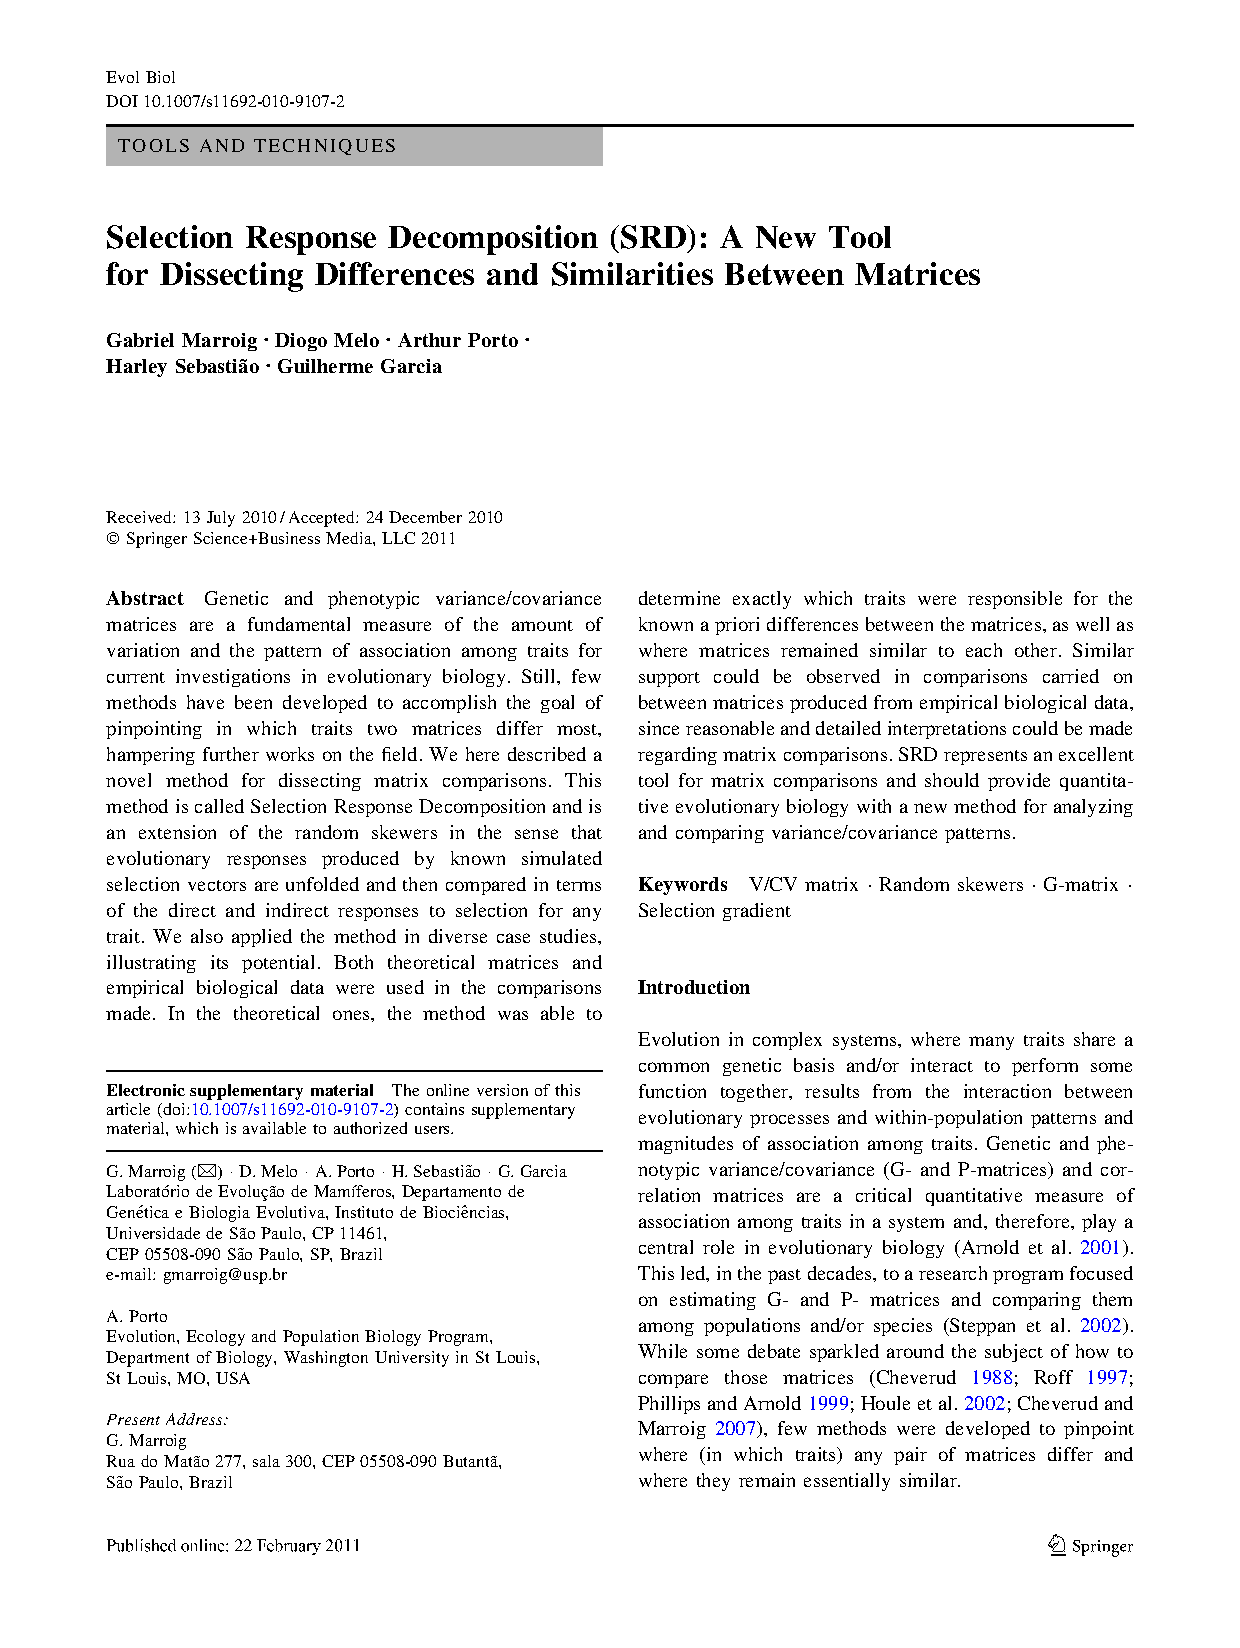
\includepdf[
            pages=-,
            width=189mm,
            height=267.3mm,
            offset=15pt 0pt,
            pagecommand={\pagestyle{plain}}
            ]{Appendix/Marroig2011.pdf}

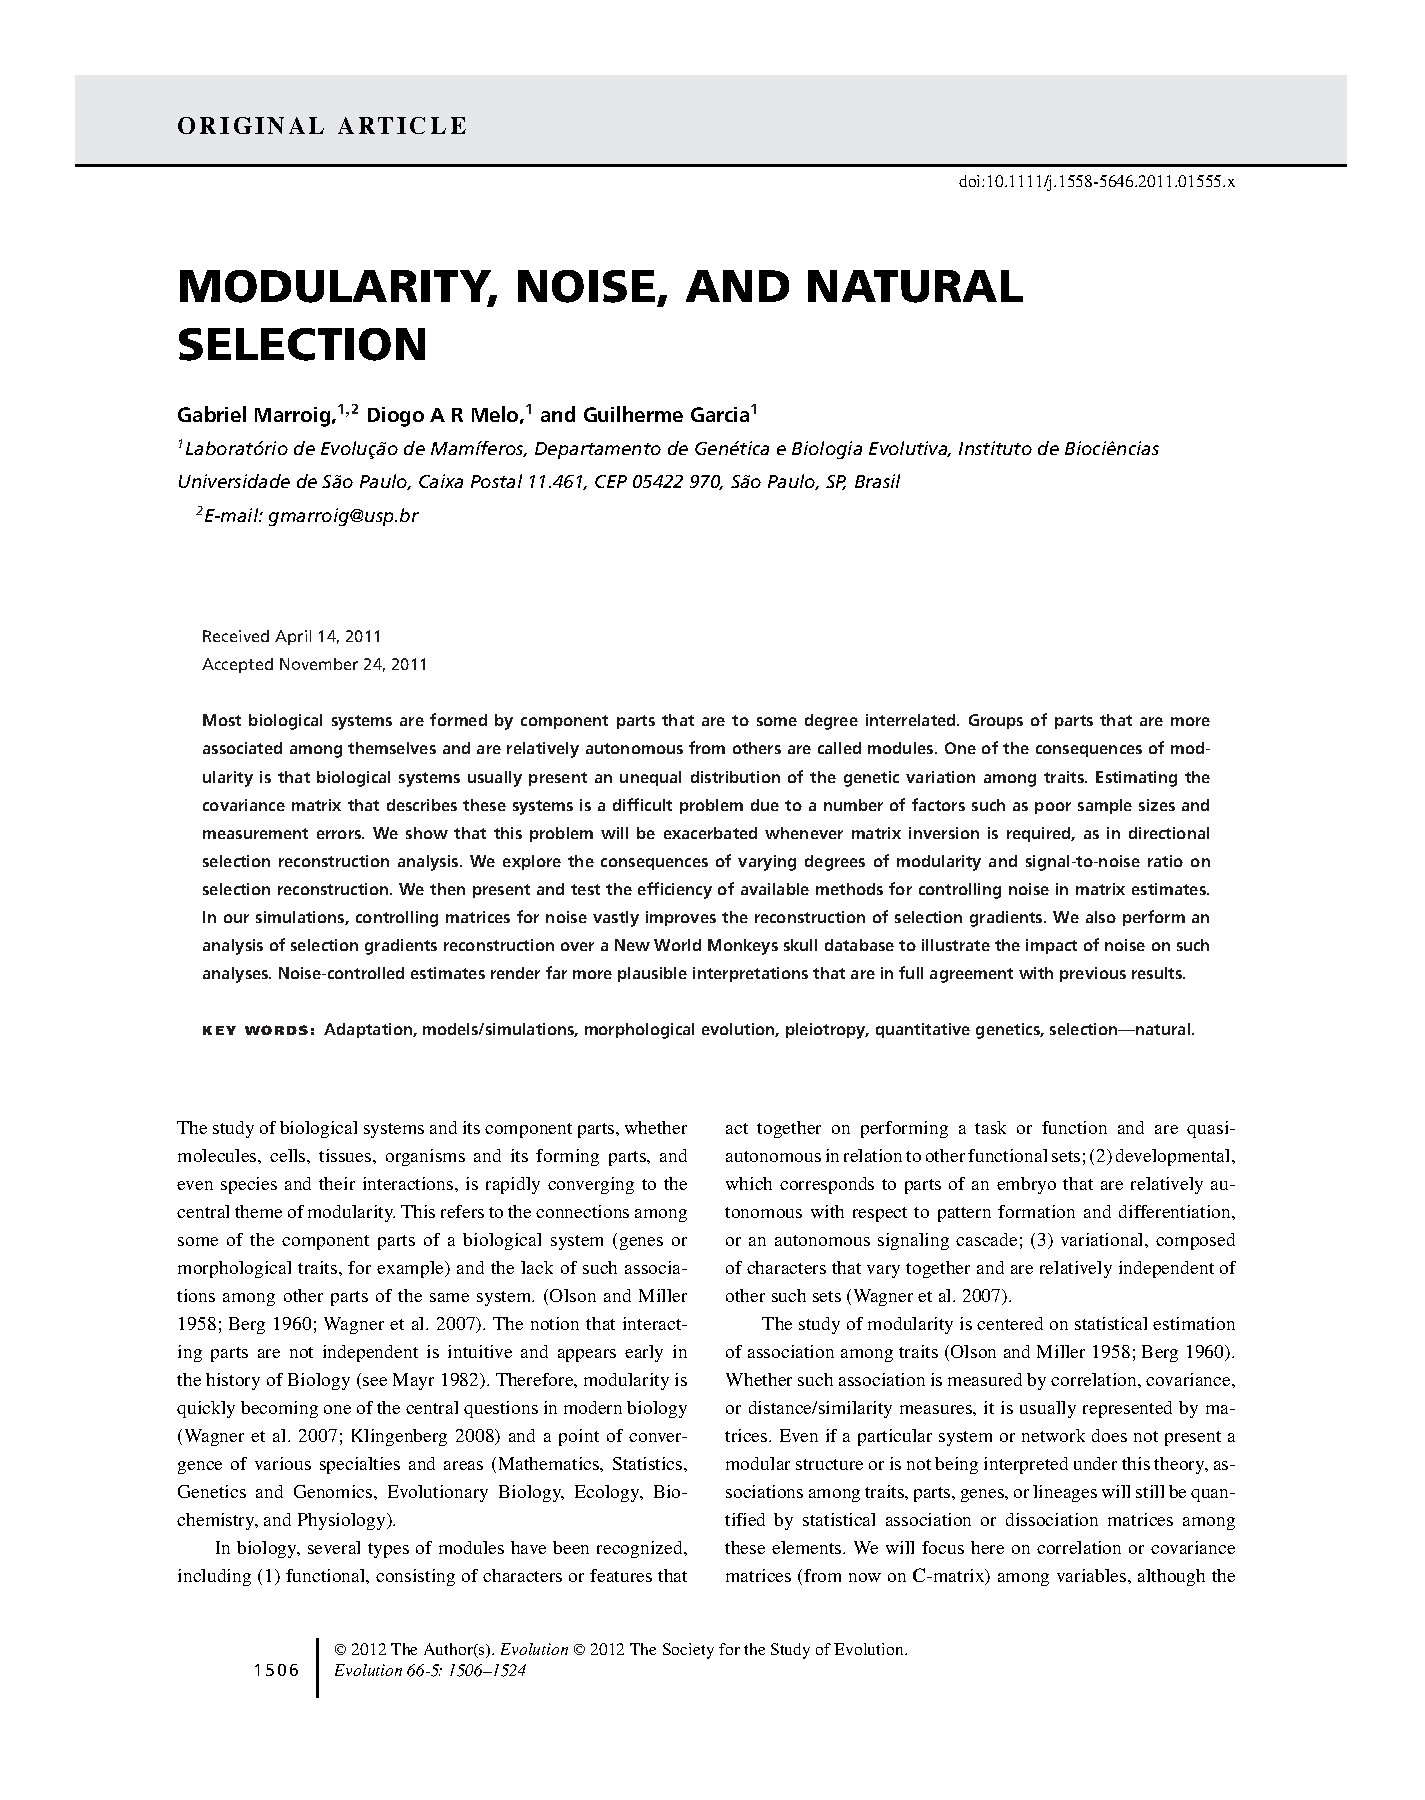
\includepdf[
            pages=-,
            width=189mm,
            height=267.3mm,
            offset=15pt 0pt,
            pagecommand={\pagestyle{plain}}
            ]{Appendix/Marroig2012.pdf}

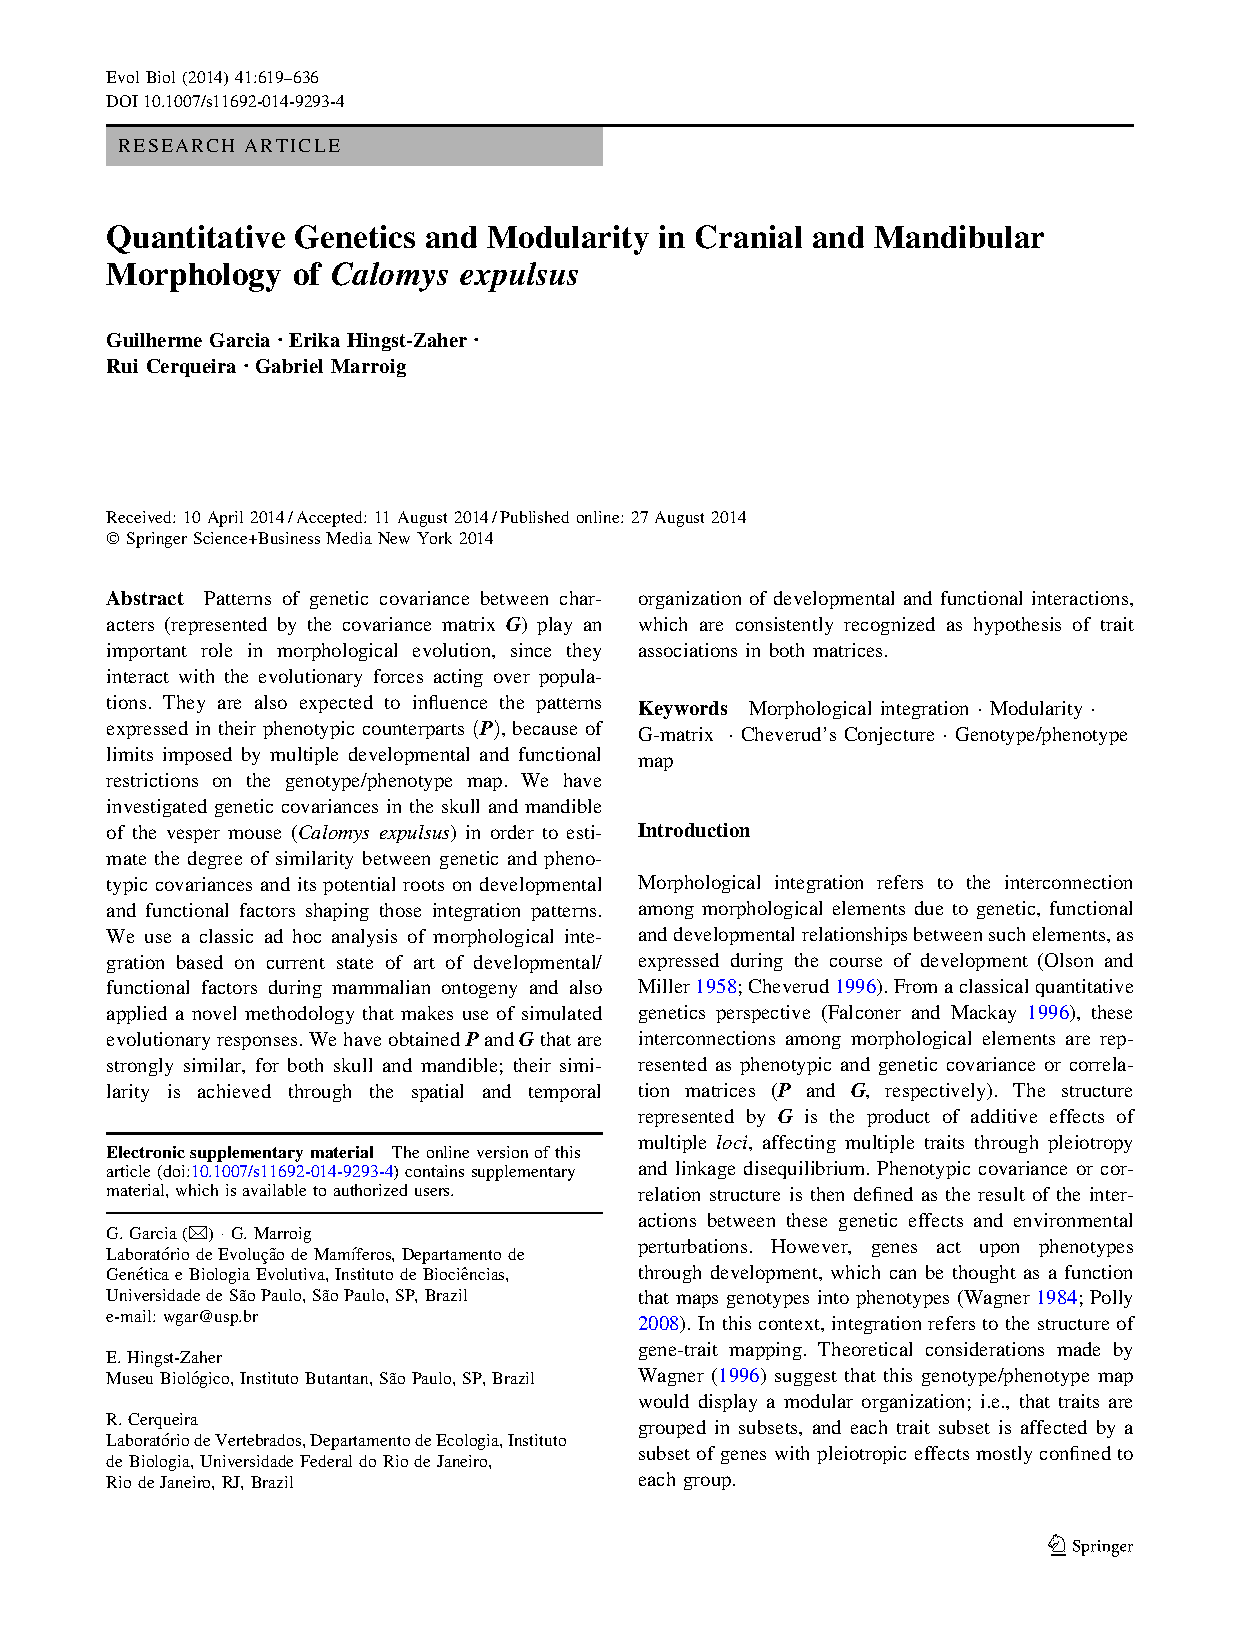
\includepdf[
            pages=-,
            width=189mm,
            height=267.3mm,
            offset=15pt 0pt,
            pagecommand={\pagestyle{plain}}            
            ]{Appendix/Garcia2014.pdf}

\end{document}
